\documentclass[12pt,a4paper]{article}

% Packages
\usepackage[utf8]{inputenc}
\usepackage[T1]{fontenc}
\usepackage[expansion=false]{microtype}
\usepackage{amsmath,amssymb,amsthm}
\usepackage{graphicx}
\usepackage{hyperref}
\usepackage{geometry}
\usepackage{natbib}
\usepackage{booktabs}
% Algorithms not available, using basic formatting
\usepackage{verbatim}
\usepackage{subcaption}
\usepackage{xcolor}
\usepackage{tikz}
\usetikzlibrary{shapes,arrows,positioning}

% Page geometry
\geometry{
  left=2.5cm,
  right=2.5cm,
  top=2.5cm,
  bottom=2.5cm
}

% Theorem environments
\newtheorem{theorem}{Theorem}[section]
\newtheorem{lemma}[theorem]{Lemma}
\newtheorem{proposition}[theorem]{Proposition}
\newtheorem{corollary}[theorem]{Corollary}

\theoremstyle{definition}
\newtheorem{definition}[theorem]{Definition}
\newtheorem{example}[theorem]{Example}

\theoremstyle{remark}
\newtheorem{remark}[theorem]{Remark}

% Title information
\title{An Ethical Riemann Hypothesis:\\
       A Formal Model for Quantifying AI Moral Fallibility\\
       under Complexity}

\author{Pei-Chen Lee \\
        National Chengchi University \\
        110462011@nccu.edu.tw}

\date{\today}

\begin{document}

\maketitle

\begin{abstract}
As artificial intelligence systems increasingly participate in moral decision-making, we urgently need rigorous frameworks to understand when and how these systems fail structurally. This paper proposes the \emph{Ethical Riemann Hypothesis} (ERH), a mathematical framework that quantifies error growth patterns in moral judgment systems through an analogy with prime number distribution in analytic number theory.

We define ``ethical primes'' as fundamental misjudgments that cannot be reduced to simpler cases, and introduce $\Pi(x)$, the counting function for ethical primes up to complexity level $x$. By establishing a baseline expectation $B(x)$ analogous to the logarithmic integral, we characterize systematic deviations through the error term $E(x) = \Pi(x) - B(x)$. The ERH states that $|E(x)| \leq C \cdot x^{1/2 + \varepsilon}$ for constants $C, \varepsilon > 0$, indicating that errors in ``healthy'' judgment systems grow at most sublinearly.

Through computational simulations comparing four judgment strategies---biased, noisy, conservative, and radical---on 2000 actions, we find that different systems exhibit markedly different error growth patterns: radical and biased judges show rapidly decreasing error terms ($\alpha < -0.4$), while noisy and conservative judges display relatively flat patterns ($\alpha \approx -0.1$). Notably, although all judges outperform the ERH-style worst-case bound in error growth patterns, the conservative judge's high mistake rate (61.1\%) reminds us that controlling error growth alone is insufficient to ensure overall judgment quality.

This framework provides quantitative criteria for evaluating AI moral judgment systems, identifying structural biases, and designing ethically robust systems, while offering new perspectives on fairness in machine learning, algorithmic accountability, and the philosophical foundations of automated moral reasoning.

\textbf{Keywords:} Ethical Riemann Hypothesis, AI Ethics, Moral Judgment, Error Analysis, AI Fairness, Prime Number Theory, Structural Bias
\end{abstract}

% ============================================
% SECTION 1: INTRODUCTION
% ============================================
\section{Introduction}
\label{sec:introduction}

\subsection{Motivation}

The challenge of moral judgment is central to both human society and artificial intelligence systems. As AI increasingly participates in decisions affecting human welfare---from criminal justice and medical diagnosis to resource allocation and content moderation---we need rigorous frameworks for understanding when and how these systems fail \citep{jobin2019,floridi2018}.

Traditional approaches to AI ethics often focus on:
\begin{itemize}
    \item \textbf{Rule-based frameworks}: Defining explicit moral rules (e.g., Asimov's Laws of Robotics)
    \item \textbf{Consequentialism}: Optimizing outcomes (e.g., utilitarian calculus)
    \item \textbf{Fairness metrics}: Measuring statistical parity, equal opportunity, calibration \citep{hardt2016,dwork2012}
\end{itemize}

While valuable, these approaches typically analyze individual cases or aggregate statistics. They provide limited insight into the \emph{structural patterns} of misjudgment: How do errors accumulate as problems become more complex? Are there fundamental misjudgments that cascade through a system? When does a judgment system become systematically unreliable?

\subsection{The Analogy with Prime Numbers}

We propose an unexpected analogy: \emph{the distribution of critical moral misjudgments resembles the distribution of prime numbers} \citep{riemann1859,edwards1974}.

In number theory:
\begin{itemize}
    \item Prime numbers are the ``atoms'' of arithmetic---irreducible building blocks
    \item Their distribution appears irregular but follows deep patterns
    \item The Riemann Hypothesis characterizes the error in counting primes
    \item This error term encodes profound information about number-theoretic structure
\end{itemize}

In moral judgment:
\begin{itemize}
    \item Some misjudgments are ``ethical primes''---fundamental errors that don't reduce to simpler cases
    \item Their distribution across complexity levels appears irregular but may follow patterns
    \item An ``Ethical Riemann Hypothesis'' could characterize the error in counting these primes
    \item This error term encodes information about the judgment system's structural health
\end{itemize}

\subsection{Contributions}

This paper makes the following contributions:

\begin{enumerate}
    \item \textbf{Mathematical Formalization}: We define action spaces, true moral values, judgment functions, and ethical primes in a rigorous mathematical framework (Section~\ref{sec:formalization}).
    
    \item \textbf{The Ethical Riemann Hypothesis}: We state ERH precisely and interpret its meaning for judgment system quality (Section~\ref{sec:erh}).
    
    \item \textbf{Computational Framework}: We develop simulation tools to test ERH empirically across different judgment systems (Section~\ref{sec:framework}).
    
    \item \textbf{Empirical Results}: We demonstrate that biased, noisy, conservative, and radical judges exhibit distinct error patterns, with some satisfying ERH and others violating it dramatically (Section~\ref{sec:results}).
    
    \item \textbf{Philosophical Implications}: We connect ERH to classical moral philosophy and discuss its implications for AI ethics (Section~\ref{sec:philosophy}).
    
    \item \textbf{AI Ethics Applications}: We discuss how ERH provides design criteria for ethically robust AI systems (Section~\ref{sec:implications}).
\end{enumerate}

\subsection{Target Audience and Use Cases}

This paper is written for researchers and practitioners across multiple domains: \textbf{AI ethics} researchers seeking quantitative frameworks for evaluating moral judgment systems, \textbf{machine learning fairness} practitioners who need to complement traditional fairness metrics with structural health indicators, \textbf{philosophy of technology} scholars interested in formal models of ethical reasoning, and \textbf{AI governance and policy} stakeholders who require actionable criteria for regulatory oversight. Readers can use the ERH framework to: (1) \emph{audit} existing AI systems for structural degradation patterns, (2) \emph{design} new systems with built-in ERH-style bounds as design constraints, and (3) \emph{govern} AI deployment through macro-level monitoring of error growth indicators. The framework provides a common quantitative language that bridges technical system evaluation and ethical assessment, enabling interdisciplinary collaboration between computer scientists, ethicists, and policymakers.

\subsection{Paper Organization}

The remainder of this paper is organized as follows. Section~\ref{sec:related} reviews related work and theoretical foundations. Section~\ref{sec:formalization} develops the mathematical formalization. Section~\ref{sec:erh} states the Ethical Riemann Hypothesis and its variants. Section~\ref{sec:framework} describes our computational framework. Section~\ref{sec:results} presents experimental results. Section~\ref{sec:philosophy} discusses philosophical implications. Section~\ref{sec:implications} discusses applications to AI ethics. Section~\ref{sec:conclusion} concludes and outlines future work.

% ============================================
% SECTION 2: RELATED WORK
% ============================================
\section{Related Work and Theoretical Foundations}
\label{sec:related}

\subsection{AI Judgment Errors and Ethical Risk}

The literature on AI ethics has extensively documented various forms of bias and unfairness in algorithmic systems \citep{mehrabi2021,barocas2016,oneil2016}. However, most approaches focus on statistical measures of fairness (e.g., demographic parity, equalized odds) or individual case analysis, rather than structural patterns of error accumulation.

\citet{binns2018} argues that fairness in machine learning should draw from political philosophy, particularly theories of distributive justice. \citet{selbst2019} emphasizes that fairness must be understood within sociotechnical systems, not as isolated algorithmic properties. While these works provide important theoretical foundations, they lack quantitative frameworks for measuring structural degradation.

\subsection{Mathematical Models in AI Ethics}

Several researchers have applied mathematical formalisms to ethical problems. \citet{dwork2012} introduced formal definitions of fairness through awareness, using metric spaces to quantify similarity. However, these approaches focus on static properties rather than dynamic error growth patterns. In formal semantics and logics of agency, Cohen and Levesque proposed a classic model that treats intention as choice with commitment \citep{cohen1990}, laying groundwork for subsequent work on deontic and intentional logics.

\subsection{Metaphorical Models in Philosophy}

The use of mathematical metaphors in philosophy has a rich history. Control theory metaphors have been applied to ethics \citep{floridi2018}, and game theory has been used to model moral dilemmas. Our approach extends this tradition by using analytic number theory as a lens for understanding moral judgment systems.

\subsection{The Riemann Hypothesis in Number Theory}

The classical Riemann Hypothesis, proposed by \citet{riemann1859}, concerns the distribution of zeros of the Riemann zeta function $\zeta(s)$. \citet{montgomery1973} showed that the pair correlation of zeros follows specific patterns, suggesting deep structure in prime distribution. \citet{granville2007} further developed connections between character sums and prime distribution.

While the Riemann Hypothesis remains unproven, its implications for prime number distribution are profound. We adapt this framework to ethical primes, recognizing that the analogy is heuristic but potentially illuminating.

\subsection{Gap Analysis}

Current approaches to AI ethics suffer from several limitations:
\begin{itemize}
    \item \textbf{Lack of structural analysis}: Most methods analyze individual cases or aggregate statistics, missing patterns of error accumulation
    \item \textbf{No complexity-aware metrics}: Existing fairness metrics don't account for how errors scale with problem complexity
    \item \textbf{Insufficient formalization}: Few frameworks provide rigorous mathematical models for ethical error patterns
    \item \textbf{Missing predictive criteria}: There are no quantitative criteria for when a judgment system becomes systematically unreliable
\end{itemize}

Our ERH framework addresses these gaps by providing a structural, complexity-aware, formally rigorous, and predictive model of ethical error patterns.

\begin{table}[htbp]
\centering
\caption{Comparison of Existing Methods with ERH Framework}
\label{tab:comparison}
\begin{tabular}{lcc}
\toprule
\textbf{Feature} & \textbf{Existing Methods} & \textbf{ERH Framework} \\
\midrule
Analysis Level & Individual/Aggregate & Structural \\
Complexity Awareness & No & Yes \\
Mathematical Rigor & Limited & High \\
Predictive Power & Low & High \\
Error Growth Model & None & Sublinear bound \\
\bottomrule
\end{tabular}
\end{table}

% --------------------------------------------
\subsection{Comparison to Reliability, Calibration, and Fairness Metrics}
\label{subsec:comparison_calibration}

Our ERH framework is closely related to, but conceptually distinct from, existing reliability and fairness metrics in machine learning.
Classical \emph{reliability} measures such as the Brier score and expected calibration error (ECE) evaluate how well predicted probabilities align with empirical frequencies on a fixed prediction task.
They are fundamentally \emph{pointwise or distributional} diagnostics: given a pool of predictions and labels, they assess whether a model is well-calibrated overall, without explicitly tracking how errors accumulate as the problem becomes more complex.

By contrast, ERH is explicitly \emph{complexity-aware}.
Instead of asking whether predictions are calibrated at a single level of difficulty, we ask how the count of fundamental misjudgments---ethical primes---grows as we move along a complexity axis.
The error term $E(x) = \Pi(x) - B(x)$ and its conjectured bound $|E(x)| \leq C x^{1/2+\varepsilon}$ provide a global constraint on how quickly structural failure can accumulate across complexity buckets.
This makes ERH particularly sensitive to long-tail, high-complexity regimes where standard calibration scores may remain acceptable while rare but catastrophic errors proliferate.

Similarly, many \emph{fairness} metrics (e.g., demographic parity, equal opportunity, calibration within groups) are defined on protected subpopulations but remain largely agnostic to how error patterns evolve with task complexity.
They tell us whether a system is fair \emph{on average} for each group, but not whether it exhibits structural degradation concentrated in high-stakes, high-complexity regions of the action space.
ERH complements these metrics by providing:
\begin{itemize}
    \item a \textbf{structural view} of misjudgment that tracks how ethical primes accumulate as complexity increases;
    \item a \textbf{growth-exponent} perspective that distinguishes systems with benign error scaling from those whose error structures explode in the tail;
    \item a \textbf{macro-level diagnostic} that can be used to compare different judgment systems---or different mitigation strategies---even when they have similar average accuracy or fairness scores.
\end{itemize}

In short, existing reliability and fairness measures characterize how a system behaves at a fixed level of difficulty or across demographic groups, whereas ERH characterizes how its \emph{structural error landscape} evolves along the complexity axis.
This distinction underlies the role of ERH as a complementary auditing tool rather than a replacement for standard metrics.

% ============================================
% SECTION 3: MODEL CONSTRUCTION
% ============================================
\section{Model Construction}
\label{sec:formalization}

\subsection{Action Space}

\begin{definition}[Action Space]
An \emph{action space} is a finite set $\mathcal{A} = \{a_1, a_2, \ldots, a_N\}$ where each action $a_i$ has the following attributes:
\begin{itemize}
    \item \textbf{Complexity} $c(a) \in \mathbb{N}$: A positive integer representing the decision's complexity (information requirements, number of stakeholders, uncertainty, etc.)
    \item \textbf{True Moral Value} $V(a) \in \mathbb{R}$: The ``ground truth'' ethical evaluation, typically normalized to $[-1, 1]$ where $-1$ is maximally harmful, $0$ is neutral, and $+1$ is maximally beneficial
    \item \textbf{Importance Weight} $w(a) \in \mathbb{R}^+$: The significance of the action (number of people affected, magnitude of consequences, etc.)
\end{itemize}
\end{definition}

\begin{remark}
The true moral value $V(a)$ represents an idealized ``god's-eye view'' or consensus among perfect moral reasoners. In practice, this is inaccessible and must be approximated. In our simulations, we define $V(a)$ explicitly as ground truth.
\end{remark}

\subsection{Judgment Systems}

\begin{definition}[Judgment System]
A \emph{judgment system} $\mathcal{J}$ is a function that assigns a moral evaluation to each action:
\[
\mathcal{J}: \mathcal{A} \to \mathbb{R}
\]
We denote $J(a) = \mathcal{J}(a)$ as the judgment of action $a$.
\end{definition}

\begin{definition}[Judgment Error]
The \emph{error} of judgment $\mathcal{J}$ on action $a$ is:
\[
\Delta(a) = J(a) - V(a)
\]
A judgment is considered a \emph{mistake} if $|\Delta(a)| > \tau$ for some threshold $\tau > 0$.
\end{definition}

We define a binary mistake indicator:
\[
M(a) = \begin{cases}
1 & \text{if } |\Delta(a)| > \tau \\
0 & \text{otherwise}
\end{cases}
\]

\subsection{Ethical Primes\index{ethical prime}}

\begin{definition}[Ethical Prime]
An action $a \in \mathcal{A}$ is an \emph{ethical prime}\index{ethical prime} if:
\begin{enumerate}
    \item $M(a) = 1$ (it is misjudged)
    \item $w(a)$ is large (high importance, typically in top quantile)
    \item $a$ is ``structurally fundamental'': correcting this error would significantly reduce overall misjudgment
\end{enumerate}
\end{definition}

Let $\mathcal{P} \subseteq \mathcal{A}$ denote the set of ethical primes. In practice, we select $\mathcal{P}$ by filtering misjudged actions by importance quantile and complexity range.

\begin{proposition}[Stability of Ethical Prime Set]
\label{prop:prime_stability}
Given an action space $\mathcal{A}$ and a judgment system $\mathcal{J}$, let the importance threshold be $w_0$. Then the ethical prime set $\mathcal{P}$ satisfies:
\[
|\mathcal{P}| \leq \min\left(|\{a \in \mathcal{A} : M(a) = 1\}|, |\{a \in \mathcal{A} : w(a) \geq w_0\}|\right)
\]
Furthermore, if the judgment system satisfies a uniform error bound $|\Delta(a)| \leq \delta$ for all $a \in \mathcal{A}$ with error threshold $\tau > \delta$, then $\mathcal{P} = \emptyset$. Conversely, if there exists some complexity level $c_0$ such that for all actions with $c(a) \geq c_0$, the probability that $|\Delta(a)| > \tau$ and $w(a) \geq w_0$ is $p > 0$, then the expected number of ethical primes is at least $p \cdot |\{a \in \mathcal{A} : c(a) \geq c_0, w(a) \geq w_0\}|$.
\end{proposition}

\begin{proof}[Proof Sketch]
The first inequality follows directly from the definition of ethical primes: they must be both mistakes ($M(a) = 1$) and high importance ($w(a) \geq w_0$). If the uniform error bound holds, then $|\Delta(a)| \leq \delta < \tau$ for all actions, so $M(a) = 0$ for all $a$, resulting in $\mathcal{P} = \emptyset$. The final expectation follows from basic probability theory: if each qualifying action becomes an ethical prime with probability $p$, the expected count is the product of probability and quantity.
\end{proof}

\subsection{Theoretical Distinction of Judge Types}

Different types of judgment systems exhibit distinct theoretical characteristics in their error structures. We can establish error bounds and expected behaviors for each type:

\begin{proposition}[Error Structure of Biased Judge]
\label{prop:biased_error}
For a biased judge with monotone increasing bias function $b(c)$ and $b(0) = 0$, noise variance $\sigma^2$, the expected error satisfies:
\[
\mathbb{E}[|\Delta(a)|] \geq |b(c(a))| - \sigma \sqrt{\frac{2}{\pi}}
\]
If $b(c) = b_0 \cdot c^\beta$ for some $b_0 > 0, \beta > 0$, then error grows with complexity, and ethical primes are more likely to occur in higher $c(a)$ ranges.
\end{proposition}

\begin{proposition}[Error Structure of Noisy Judge]
\label{prop:noisy_error}
For a noisy judge with noise variance $\sigma^2(c)$ that may vary with complexity, the variance of error is:
\[
\text{Var}[\Delta(a)] = \sigma^2(c(a))
\]
If $\sigma(c) = \sigma_0 \cdot c^\gamma$ for $\sigma_0 > 0, \gamma \geq 0$, then high-complexity cases have larger error variability. When $\gamma > 0$, the error growth exponent $\alpha$ tends toward $0$, as error is primarily dominated by randomness rather than systematic patterns.
\end{proposition}

\begin{proposition}[Error Structure of Conservative Judge]
\label{prop:conservative_error}
For a conservative judge with shrinkage factor $\lambda(c) \in [0,1]$ that increases monotonically with complexity, the expected error is approximately:
\[
\mathbb{E}[|\Delta(a)|] \approx |V(a)| \cdot \lambda(c(a))
\]
The conservative strategy causes all judgments to shrink toward neutral, so low-complexity cases ($|V(a)|$ near $1$) may exhibit large errors, while high-complexity ambiguous cases ($|V(a)| \approx 0$) have small errors. This explains why conservative judges have the highest mistake rate but near-zero error growth exponent.
\end{proposition}

\begin{proposition}[Error Structure of Radical Judge]
\label{prop:radical_error}
For a radical judge with amplification factor $\alpha > 1$, the error is:
\[
\Delta(a) = (\alpha - 1) \cdot V(a) + \mathcal{N}(0, \sigma^2)
\]
When $|V(a)|$ is large, amplification causes significant errors; when $|V(a)| \approx 0$, error is primarily dominated by noise. Thus radical judges perform poorly on low-complexity clear cases but may provide clearer discriminative signals in high-complexity ambiguous cases, leading to decreasing error as complexity increases.
\end{proposition}

\subsection{Counting Functions}

\begin{definition}[Ethical Prime Counting Function]
Define $\Pi(x)$ as the number of ethical primes with complexity at most $x$:
\[
\Pi(x) = \#\{p \in \mathcal{P} : c(p) \leq x\}
\]
\end{definition}

\begin{definition}[Baseline Function]
The \emph{baseline function} $B(x)$ represents the expected number of ethical primes up to complexity $x$ under some smooth model. We consider several forms:
\begin{enumerate}
    \item \textbf{Linear}: $B(x) = \alpha x$ for some $\alpha > 0$
    \item \textbf{Prime Theorem Analog}: $B(x) = \beta \frac{x}{\log x}$ for some $\beta > 0$, directly analogous to the Prime Number Theorem
    \item \textbf{Logarithmic Integral}: $B(x) = \beta \cdot \text{Li}(x)$ where $\text{Li}(x) = \int_2^x \frac{dt}{\log t}$
    \item \textbf{Power Law}: $B(x) = \gamma x^\delta$ for parameters $\gamma, \delta > 0$
\end{enumerate}
\end{definition}

\begin{definition}[Error Term]
The \emph{error term} is:
\[
E(x) = \Pi(x) - B(x)
\]
This measures how the actual distribution of ethical primes deviates from the baseline expectation.
\end{definition}

\subsection{Example: Computing $\Pi(x)$}

Consider a simple example with three actions:
\begin{itemize}
    \item $a_1$: $c(a_1) = 5$, $V(a_1) = 0.8$, $w(a_1) = 10$, $|\Delta(a_1)| = 0.4$ (mistake)
    \item $a_2$: $c(a_2) = 15$, $V(a_2) = -0.6$, $w(a_2) = 8$, $|\Delta(a_2)| = 0.5$ (mistake)
    \item $a_3$: $c(a_3) = 20$, $V(a_3) = 0.3$, $w(a_3) = 12$, $|\Delta(a_3)| = 0.2$ (not a mistake)
\end{itemize}

If $\tau = 0.3$ and we select ethical primes as top 50\% by importance among mistakes, then $\mathcal{P} = \{a_1, a_2\}$ (both are mistakes, and $a_1$ has highest importance). Then:
\begin{align*}
\Pi(10) &= 1 \quad \text{(only $a_1$ has $c \leq 10$)} \\
\Pi(15) &= 2 \quad \text{(both $a_1$ and $a_2$ have $c \leq 15$)} \\
\Pi(20) &= 2 \quad \text{(both have $c \leq 20$)}
\end{align*}

% ============================================
% SECTION 4: THE ETHICAL RIEMANN HYPOTHESIS
% ============================================
\section{The Ethical Riemann Hypothesis}
\label{sec:erh}

\subsection{Statement of ERH}

\begin{theorem}[Ethical Riemann Hypothesis (ERH)]
\label{thm:erh}
Let $\mathcal{J}$ be a judgment system and let $E(x) = \Pi(x) - B(x)$ be the error term for its ethical prime distribution. The judgment system satisfies the \emph{Ethical Riemann Hypothesis} if there exist constants $C, \varepsilon > 0$ such that:
\[
|E(x)| \leq C \cdot x^{1/2 + \varepsilon}
\]
for all $x$ in the complexity range. This bound $|E(x)| \leq C \cdot x^{1/2 + \varepsilon}$ is called the \emph{ERH-style bound}\index{ERH-style bound}.
\end{theorem}

\begin{remark}[ERH as an Empirical Diagnostic Hypothesis]
\label{rem:erh_empirical}
In contrast to the classical Riemann Hypothesis, we do \emph{not} claim to prove or refute ERH as a formal theorem about an underlying mathematical object. Throughout this paper, ERH is treated as an \emph{empirical diagnostic hypothesis}: an ideal error-growth bound inspired by analytic number theory, against which we test concrete (simulated or real-world) judgment systems. Our contribution is to propose this ERH-style bound as a diagnostic lens and to develop computational tools that estimate error growth and check whether observed systems are consistent with the bound within reasonable finite-sample slack.
\end{remark}

\begin{remark}[ERH as a Necessary but Not Sufficient Condition]
\label{rem:erh_necessary}
The ERH-style bound $|E(x)| \leq C \cdot x^{1/2 + \varepsilon}$ provides a \emph{necessary condition} for structural health of a judgment system: it ensures that error growth remains sublinear and bounded. However, satisfying this bound alone is \emph{not sufficient} to guarantee that a system is morally acceptable. A judgment system must also maintain low overall error rates and avoid systematic biases. As demonstrated in our experimental results (Section~\ref{sec:results}), a system can satisfy the ERH-style bound while still exhibiting unacceptably high mistake rates (e.g., the Conservative Judge with 61.1\% mistake rate). Therefore, the ERH-style bound should be evaluated alongside other metrics such as overall accuracy, fairness measures, and domain-specific quality criteria.
\end{remark}

\subsection{Intuitive Interpretation}

The ERH states that the cumulative error in predicting critical misjudgments grows at most like $\sqrt{x}$ (up to a small factor $x^\varepsilon$). This is a \emph{sublinear} growth rate, meaning:

\begin{itemize}
    \item As problem complexity increases, the judgment system doesn't lose control
    \item Errors accumulate slowly and predictably
    \item The system maintains structural integrity across scales
\end{itemize}

\subsection{Probabilistic Setting}
\label{subsec:prob_setting}

To connect ERH with a probabilistic view of judgment systems, we model ethical prime generation as a random process over complexity levels.
For each integer complexity level $c \in \{1,2,\dots\}$, let $N(c)$ denote the (possibly random) number of actions with complexity exactly $c$, and let
\[
X_c = \#\{a \in \mathcal{A} : c(a)=c,\ a \text{ is an ethical prime}\}
\]
be the random number of ethical primes at complexity $c$.
Then the cumulative prime count and baseline can be written as
\[
\Pi(x) = \sum_{c \le x} X_c,
\qquad
B(x) = \sum_{c \le x} \mu_c,
\]
where $\mu_c = \mathbb{E}[X_c]$ is the expected number of ethical primes at level $c$ under some smooth generative model.
The error term becomes
\[
E(x) = \sum_{c \le x} (X_c - \mu_c).
\]

We make the following assumptions:
\begin{itemize}
    \item[(A1)] (\emph{Controlled growth of candidate actions}) There exist constants $C_0,d > 0$ such that almost surely
    \[
    0 \le X_c \le N(c) \le C_0 c^d
    \quad \text{for all } c \ge 1.
    \]
    \item[(A2)] (\emph{Decaying prime rate}) There exist constants $C_1,\beta > 0$ such that
    \[
    \mu_c = \mathbb{E}[X_c] \le C_1 c^{-\beta} N(c)
    \quad \text{for all sufficiently large } c.
    \]
    Intuitively, the probability that a high-complexity action becomes an ethical prime decays as a power of $c$.
    \item[(A3)] (\emph{Approximate independence}) Conditional on $N(c)$, the variables $X_c$ are independent across complexities, and each $X_c$ can be viewed as a sum of at most $N(c)$ bounded contributions (e.g., Bernoulli indicators for each action).
\end{itemize}

Assumptions (A1)--(A3) capture the idea that while there may be many high-complexity actions, ethical primes become increasingly rare, and prime occurrences at different complexity levels do not exhibit pathological long-range dependence.

\subsection{A Non-trivial Probabilistic Theorem}
\label{subsec:prob_theorem}

Under the probabilistic setting above, we can show that ERH-type bounds arise naturally when ethical primes become sufficiently rare at high complexity.

\begin{theorem}[Probabilistic ERH Bound under Decaying Prime Rate]
\label{thm:prob_erh}
Suppose (A1)--(A3) hold with parameters $C_0,d,C_1,\beta>0$.
Assume moreover that $\beta > 1$ and that for some $\varepsilon \in (0, \tfrac{\beta-1}{2})$ the following variance bound holds:
\[
\operatorname{Var}(X_c) \le C_2 c^{d-\beta}
\quad \text{for all sufficiently large } c
\]
for a constant $C_2>0$.
Then there exists a constant $C>0$ (depending on $C_0,C_1,C_2,d,\beta,\varepsilon$) such that with probability at least $1 - O(x^{-\varepsilon})$ we have
\[
|E(x)| \le C\, x^{1/2+\varepsilon}
\quad \text{for all sufficiently large } x.
\]
In particular, under these assumptions the judgment system satisfies an ERH-type sublinear growth bound for the error term with high probability.
\end{theorem}

\begin{proof}[Proof Sketch]
Write $Y_c = X_c - \mu_c$, so that $E(x) = \sum_{c \le x} Y_c$ and $\mathbb{E}[Y_c]=0$.
By (A1) and (A2), $|Y_c| \le X_c + \mu_c \le 2 C_0 c^d$ for all large $c$, and by the variance assumption we have
\[
\sum_{c \le x} \operatorname{Var}(Y_c)
 = \sum_{c \le x} \operatorname{Var}(X_c)
 \le C_2 \sum_{c \le x} c^{d-\beta}
 = O(x^{d-\beta+1}).
\]
Since $\beta>1$, the exponent $d-\beta+1$ is strictly less than $d$.

Using Bernstein's inequality (or another standard concentration inequality for sums of independent, bounded random variables), for any $t>0$ we obtain
\[
\mathbb{P}\big(|E(x)| \ge t\big)
\le 2 \exp\left(
 - \frac{t^2/2}{\sum_{c \le x} \operatorname{Var}(Y_c) + M t}
\right),
\]
where $M$ is a bound on $|Y_c|$.
Substituting the bounds above and choosing $t = K x^{1/2+\varepsilon}$ for a suitable constant $K>0$, the exponent becomes polynomially small in $x$ provided $\varepsilon < (\beta-1)/2$.
Thus we obtain
\[
\mathbb{P}\big(|E(x)| \ge K x^{1/2+\varepsilon}\big)
 = O(x^{-\varepsilon})
\]
for large $x$.
Applying a union bound over dyadic scales of $x$ yields the claimed high-probability bound for all sufficiently large $x$ simultaneously.
\end{proof}

This theorem is intentionally modest in scope: it does not claim that all reasonable judgment systems must satisfy ERH, but rather that \emph{under explicit probabilistic assumptions about how ethical primes thin out at high complexity}, an ERH-type bound on $E(x)$ follows from standard concentration arguments.
In this sense, ERH can be understood as a mathematically natural regularity condition for judgment systems whose structural failures do not explode in the tail.

\subsection{Comparison with Classical Riemann Hypothesis}

\begin{table}[htbp]
\centering
\caption{Analogy between Classical RH and ERH}
\label{tab:analogy}
\begin{tabular}{ll}
\toprule
\textbf{Number Theory} & \textbf{Ethical Judgment} \\
\midrule
Natural number $n$ & Action complexity $c$ \\
Prime $p$ & Ethical prime (critical misjudgment) \\
$\pi(x)$ (prime counting) & $\Pi(x)$ (ethical prime counting) \\
$\text{Li}(x) \sim \frac{x}{\log x}$ & $B(x) \sim \frac{x}{\log x}$ \\
$E(x) = \pi(x) - \text{Li}(x)$ & $E(x) = \Pi(x) - B(x)$ \\
RH: $|E(x)| = O(x^{1/2} \log x)$ & ERH: $|E(x)| = O(x^{1/2 + \varepsilon})$ \\
$\zeta(s)$ Riemann zeta function & $\zeta_E(s)$ Ethical zeta function \\
Zeros of $\zeta(s)$ & Zeros of $\zeta_E(s)$ \\
\bottomrule
\end{tabular}
\end{table}

\subsection{Ethical Zeta Function}

We can define an ``ethical zeta function'' via generating functions:

\begin{definition}[Ethical Zeta Function]
Let $m(n)$ be the number (or weighted count) of ethical primes at complexity level $n$. Define:
\[
\zeta_E(s) = \sum_{n=1}^{N} \frac{m(n)}{n^s}
\]
for $s \in \mathbb{C}$ with $\text{Re}(s) > 1$.
\end{definition}

\subsection{Analytic Properties of the Ethical Zeta Function}

Although the ethical zeta function $\zeta_E(s)$ is a finite sum (unlike the infinite series of the classical Riemann zeta function), we can still analyze its basic analytic properties and establish heuristic connections with the error term $E(x)$.

\begin{proposition}[Domain of Convergence and Analyticity]
\label{prop:zeta_convergence}
The ethical zeta function $\zeta_E(s)$ is defined for all $s \in \mathbb{C}$ (since it is a finite sum), but it exhibits structural characteristics similar to the classical zeta function in the region $\text{Re}(s) > 1$. If $m(n) = O(n^\delta)$ for some $\delta < 1$, then in the region $\text{Re}(s) > \delta + 1$, the growth of $\zeta_E(s)$ is primarily dominated by low-complexity terms.
\end{proposition}

\begin{proposition}[Heuristic Connection between Zero Distribution and Error Term]
\label{prop:zeros_error_heuristic}
(Heuristic, non-rigorous) If the zeros of the ethical zeta function $\zeta_E(s)$ cluster near some critical line (e.g., $\text{Re}(s) = \sigma_0$), then the growth rate of the error term $E(x)$ may relate to $\sigma_0$:
\[
|E(x)| \sim x^{\sigma_0} \quad \text{(heuristic)}
\]
Specifically, if zeros cluster near $\text{Re}(s) = 1/2$, this may indicate that $|E(x)| = O(x^{1/2 + \varepsilon})$, consistent with the ERH-style worst-case bound. This is a heuristic analogy rather than a rigorous theorem, as the connection between zeros of the classical zeta function and the error term in prime distribution involves sophisticated analytic number theory techniques (such as Perron's formula and Mellin transforms), which our finite-sum version does not possess to the same degree of theoretical structure.
\end{proposition}

\begin{remark}[Heuristic Value and Limitations of the Analogy]
The analogy between the ethical zeta function and the classical Riemann zeta function has heuristic value but important differences:
\begin{itemize}
    \item \textbf{Finitude}: $\zeta_E(s)$ is a finite sum, so there is no analytic continuation, functional equation, or critical strip concept, which are key features of the classical zeta function.
    \item \textbf{Structural differences}: The distribution of ethical primes may not possess the deep number-theoretic structure of prime distribution (such as the prime number theorem in arithmetic progressions).
    \item \textbf{Heuristic value}: Nevertheless, zero analysis may still reveal periodic patterns in error distribution, and spectral analysis (corresponding to discrete Fourier transform) can identify correlations between complexity levels.
\end{itemize}
\end{remark}

The distribution of zeros of $\zeta_E(s)$ in the complex plane encodes information about the ``periodicity'' or ``regularity'' of ethical prime distribution. If zeros cluster near a critical line (analogous to $\text{Re}(s) = 1/2$ for the Riemann zeta), this suggests deep structural regularity in the judgment errors. However, we must recognize this as a heuristic analogy rather than a rigorous number-theoretic correspondence.

% ============================================
% SECTION 5: SIMULATION SETUP
% ============================================
\section{Simulation Design and Experimental Methods}
\label{sec:framework}

\subsection{Action Space Generation}

We generate actions with complexity sampled from:
\begin{itemize}
    \item \textbf{Uniform distribution}: $c(a) \sim \text{Uniform}(1, C_{\max})$
    \item \textbf{Zipf distribution}: $c(a) \sim \text{Zipf}(\alpha)$ (more realistic, many simple cases, few complex)
    \item \textbf{Power law}: $c(a) \sim x^{-\gamma}$
\end{itemize}

True moral values $V(a)$ are generated with \emph{complexity-dependent ambiguity}:
\begin{itemize}
    \item Low complexity: clear values (near $\pm 1$)
    \item High complexity: ambiguous values (near $0$)
\end{itemize}

This reflects the intuition that simple moral cases are often clear-cut, while complex cases involve multiple competing considerations.

\subsection{Judgment System Models}

We implement five archetypal judges:

\begin{enumerate}
    \item \textbf{BiasedJudge}: Systematic bias $b(c)$ increasing with complexity:
    \[
    J(a) = V(a) + b_0 \cdot f(c(a)) + \mathcal{N}(0, \sigma^2)
    \]
    where $f(c)$ is monotone increasing.
    
    \item \textbf{NoisyJudge}: High random noise:
    \[
    J(a) = V(a) + \mathcal{N}(0, \sigma^2(c))
    \]
    where noise scales with complexity.
    
    \item \textbf{ConservativeJudge}: Shrinks toward neutral:
    \[
    J(a) = (1-\lambda(c)) V(a) + \mathcal{N}(0, \sigma^2)
    \]
    where $\lambda(c) \in [0,1]$ increases with complexity.
    
    \item \textbf{RadicalJudge}: Amplifies extremes:
    \[
    J(a) = \alpha \cdot V(a) + \mathcal{N}(0, \sigma^2)
    \]
    where $\alpha > 1$.
    
    \item \textbf{QuantumJudge}: Superposition-based judgment via quantum measurement. Let $\theta = c(a)/100 \cdot \pi$; apply Rx$(\theta)$ rotation to $|0\rangle$. Measurement yields $J(a) = 2|\alpha|^2 - 1 \in [-1, 1]$, where $|\alpha|^2$ is the probability of measuring ``ethical'' ($|0\rangle$). Uses qiskit-aer when available; otherwise NumPy fallback for deterministic reproducibility.
\end{enumerate}

\subsection{Analysis Pipeline}

For each judgment system:
\begin{enumerate}
    \item Generate action space with $N = 2000$ actions
    \item Evaluate all actions with judge $\mathcal{J}$
    \item Compute errors $\Delta(a)$ and identify mistakes
    \item Select ethical primes $\mathcal{P}$ (top 10\% by importance)
    \item Compute $\Pi(x)$, $B(x)$, $E(x)$ for $x \in [1, 100]$
    \item Fit power law: $|E(x)| \sim C x^\alpha$
    \item Test if $\alpha \approx 0.5$ (ERH satisfied)
\end{enumerate}

\subsection{Parameter Settings}

\begin{table}[htbp]
\centering
\caption{Simulation Parameters}
\label{tab:parameters}
\begin{tabular}{lc}
\toprule
\textbf{Parameter} & \textbf{Value} \\
\midrule
Number of actions ($N$) & 2000 \\
Complexity range & [1, 100] \\
Complexity distribution & Zipf($\alpha=2.0$) \\
Error threshold ($\tau$) & 0.3 \\
Importance quantile for primes & 0.9 \\
$X_{\max}$ for analysis & 100 \\
Random seed & 42 \\
\bottomrule
\end{tabular}
\end{table}

\subsection{Reproducibility and Statistical Stability}

To ensure experimental reproducibility, we adopted the following measures:

\begin{itemize}
    \item \textbf{Fixed random seed}: All simulations use a fixed random seed ($seed = 42$), ensuring consistency in action space generation, noise generation, and judgment evaluation.
    \item \textbf{Parameter documentation}: All judge types and their parameter settings (as shown in Table~\ref{tab:parameters}) are explicitly documented for reproducibility and verification.
    \item \textbf{Action generation process}: Action space generation follows these steps:
    \begin{enumerate}
        \item Complexity $c(a)$ is sampled from a Zipf distribution: $c(a) \sim \text{Zipf}(\alpha=2.0)$ with range $[1, 100]$
        \item True moral values $V(a)$ are generated with complexity-dependent ambiguity: $V(a) = \text{sign}(\mathcal{N}(0,1)) \cdot \min(1, |\mathcal{N}(0,1)| \cdot (1 - c(a)/100))$, where low-complexity cases ($c(a) \approx 1$) tend toward $\pm 1$, and high-complexity cases ($c(a) \approx 100$) tend toward $0$
        \item Importance weights $w(a)$ are sampled from a log-normal distribution: $\log w(a) \sim \mathcal{N}(\mu=2, \sigma=1)$, ensuring a few actions have high importance
    \end{enumerate}
    \item \textbf{Judge system implementation details}:
    \begin{itemize}
        \item \textbf{Biased Judge}: $J(a) = V(a) + 0.2 \cdot (c(a)/100)^2 + \mathcal{N}(0, 0.1^2)$, bias grows quadratically with complexity
        \item \textbf{Noisy Judge}: $J(a) = V(a) + \mathcal{N}(0, (0.3 \cdot \sqrt{c(a)/100})^2)$, noise standard deviation grows with square root of complexity
        \item \textbf{Conservative Judge}: $J(a) = (1 - 0.5 \cdot c(a)/100) \cdot V(a) + \mathcal{N}(0, 0.1^2)$, shrinkage factor increases linearly with complexity
        \item \textbf{Radical Judge}: $J(a) = 1.5 \cdot V(a) + \mathcal{N}(0, 0.1^2)$, fixed amplification factor
        \item \textbf{Quantum Judge}: Rx$(\theta)$ with $\theta = c(a)/100 \cdot \pi$, shots=512; qiskit-aer or NumPy fallback
    \end{itemize}
    \item \textbf{Error growth exponent fitting}: We fit $|E(x)| \sim C x^\alpha$ using linear regression in log-log scale, where $\alpha$ is the error growth exponent. Fitting is performed over $x \in [10, 100]$ (excluding low-complexity region to reduce small-sample effects), using least squares estimation. We also report bootstrap confidence intervals for $\alpha$ obtained by resampling the $(x, |E(x)|)$ pairs, and we treat $R^2$ as a supplementary diagnostic rather than a primary model selection criterion.
    \item \textbf{Experimental repeatability}: Although the figures in the main text are based on a single representative run, we verified statistical stability across independent runs with $200$ different random seeds. For each judge, we re-estimate the growth exponent $\alpha$ across all seeds and compute mean, standard deviation, coefficient of variation (CV), and empirical 95\% confidence intervals. The CV of $\alpha$ remains below $0.15$ for all judges and the confidence intervals are narrow, indicating good consistency. Table~\ref{tab:seed_stability} summarizes the stability metrics across multiple random seeds.
\end{itemize}

\begin{table}[htbp]
\centering
\caption{Statistical stability of error growth exponent $\alpha$ across multiple random seeds. All judges exhibit low coefficient of variation (CV < 0.15), indicating stable growth exponents across random seeds.}
\label{tab:seed_stability}
\begin{tabular}{lccc}
\toprule
\textbf{Judge Type} & \textbf{mean($\alpha$)} & \textbf{std($\alpha$)} & \textbf{CV} \\
\midrule
Biased       & $-0.629$ & $0.042$ & $0.067$ \\
Noisy        & $-0.171$ & $0.018$ & $0.105$ \\
Conservative & $-0.046$ & $0.005$ & $0.109$ \\
Radical      & $-0.452$ & $0.031$ & $0.069$ \\
\bottomrule
\end{tabular}
\end{table}

\subsection{User Study of ERH Visualizations}

To assess whether our ERH-style plots are interpretable for humans, we conducted a small visualization usability check with eight technically trained participants (graduate students and engineers). Participants were shown pairs of judges and parameter settings using our error-growth plots (including $\alpha$ and bound-violation indicators) and were asked to (i) rank which judge exhibits higher long-tail risk and (ii) identify which parameter setting appears most structurally fragile. Across all trials, participants' rankings agreed with the ordering induced by our ERH metrics in 87.5\% of cases, and the median interpretability rating of the plots was 4 out of 5 on a Likert scale.

These results suggest that ERH-style visualizations are not only mathematically well-defined but also usable as risk-communication tools for practitioners. In particular, the combination of growth exponents, ERH-style bound satisfaction, and long-tail error profiles enables users to distinguish between judges that have similar average accuracy and fairness scores but very different structural error behaviors.

\subsection{Ethical Considerations}

Our simulations operate on synthetic action spaces and anonymized, tabular real-world case studies with no personal identifiers or sensitive free text. The framework evaluates \emph{judgment rules} (e.g., abstract ``judges'') rather than individual people, and all fairness-related analyses are performed at an aggregate group level. Nevertheless, ERH-style diagnostics could be misused if treated as a single scalar ``fairness score'' for high-stakes deployment decisions. We therefore recommend using ERH metrics only as diagnostic tools, in conjunction with established fairness and accountability criteria, and not as certification mechanisms. All code and configuration files necessary to reproduce our experiments (including hyperparameters, random seeds, and dataset preprocessing steps) are provided in the public repository accompanying this paper.

All judges exhibit low coefficient of variation (CV < 0.15), indicating stable growth exponents across random seeds. This demonstrates that the observed error growth patterns are robust to random initialization and not artifacts of a particular seed choice.

\subsection{Data and Code Availability}

Complete code, simulation scripts, and generated figures for this study are publicly available to promote reproducibility and further research:

\begin{itemize}
    \item \textbf{Code repository}: All simulation code, analysis scripts, and visualization tools are available in a public GitHub repository: \url{https://github.com/dennislee928/Ethic-Latex}. For reviewers, the file \texttt{docs/EXPERIMENT\_REPORTS.md} and the folder \texttt{simulation/output/} can be treated as the primary supplementary material bundle. In particular, the consolidated experiment report \texttt{docs/EXPERIMENT\_REPORTS.md} summarizes key numerical results and links to the underlying outputs.
    \item \textbf{Data outputs}: Numerical results from simulations (including statistical metrics for each judge, error term sequences, spectrum data, stability-of-$\alpha$ tables across random seeds, quantum Hilbert space metrics, etc.) are saved in the \texttt{simulation/output/} directory, including:
    \begin{itemize}
        \item \texttt{results\_summary.txt}: Statistical summary for all judges
        \item \texttt{judge\_comparison\_report.md}: Detailed comparison report
        \item \texttt{spectrum\_data.json} and \texttt{zeros\_data.json}: Spectrum and zero analysis data
        \item \texttt{quantum\_hilbert\_results.json}: Consensus state, system coherence, Von Neumann entropy from quantum Hilbert space simulation
        \item \texttt{*.csv}: Parameter sensitivity analysis results
    \end{itemize}
    \item \textbf{Figure generation}: All paper figures are automatically generated by \texttt{simulation/generate\_all\_figures.py} and \texttt{scripts/run\_quantum\_hilbert\_figures.py}. PDF figures are saved in \texttt{simulation/output/figures/}; quantum circuit and distribution PNGs (\texttt{latest\_quantum\_circuit.png}, \texttt{latest\_quantum\_distribution.png}) are produced by the quantum Hilbert simulation.
    \item \textbf{Environment dependencies}: All necessary Python packages are listed in \texttt{requirements.txt}, with Python 3.10 or higher recommended. Main dependencies include: numpy, scipy, matplotlib, pandas, jupyter (for notebook versions).
    \item \textbf{Verification and reproduction}: Readers can reproduce experiments by executing:
    \begin{verbatim}
    cd simulation
    export PYTHONPATH=$PYTHONPATH:$(pwd)
    python generate_all_figures.py
    \end{verbatim}
    or use the provided Jupyter notebooks (\texttt{simulation/notebooks/}) for interactive exploration.
\end{itemize}

\subsection{Real-World Data Acquisition}
\label{subsec:real_world_data}

Real-data case studies (Adult Income, COMPAS) require datasets that are not bundled in the repository. Table~\ref{tab:real_data_sources} lists the data sources and output paths.

\begin{table}[htbp]
\centering
\caption{Real-world data sources, URLs, and output paths}
\label{tab:real_data_sources}
\begin{tabular}{lll}
\toprule
\textbf{Dataset} & \textbf{Source} & \textbf{Output Path} \\
\midrule
Adult Income (train) & UCI ML Repository & \texttt{data/real\_world/adult.data} \\
Adult Income (test) & UCI ML Repository & \texttt{data/real\_world/adult.test} \\
Adult Income (processed) & --- & \texttt{data/adult.csv} (after conversion) \\
COMPAS & ProPublica GitHub & \texttt{data/compas-scores-two-years.csv} \\
\bottomrule
\end{tabular}
\end{table}

\textbf{Fetch and conversion steps}:
\begin{enumerate}
    \item Run \texttt{scripts/fetch\_real\_data.sh} to download Adult (\url{https://archive.ics.uci.edu/ml/machine-learning-databases/adult/}) and COMPAS (\url{https://github.com/propublica/compas-analysis}) into \texttt{data/}.
    \item Run \texttt{scripts/convert\_adult\_to\_csv.py} to convert UCI Adult format (no header, comma-separated) into \texttt{data/adult.csv} with column headers; rows containing missing values (\texttt{?}) are dropped.
\end{enumerate}

\textbf{Output paths and case study mapping}:
\begin{itemize}
    \item \texttt{data/adult.csv} $\rightarrow$ \texttt{simulation/real\_data/adult\_income\_case\_study.py} (requires \texttt{income} column)
    \item \texttt{data/compas-scores-two-years.csv} $\rightarrow$ \texttt{simulation/real\_data/compas\_case\_study.py} (requires \texttt{two\_year\_recid}, \texttt{decile\_score} columns)
\end{itemize}

\subsection{Fourier Spectrum Analysis}

To detect periodic patterns in misjudgments, we compute:
\[
\hat{m}(k) = \sum_{n=1}^{N} m(n) e^{-2\pi i kn / N}
\]
Peaks in $|\hat{m}(k)|$ indicate periodic clustering of errors at specific complexity scales.

\subsection{The Quantum Isomorphism: Transverse-Field Ising Model}
\label{sec:quantum_ising}

We model the social moral consensus system as a \emph{Transverse-Field Ising Model}. The total energy (Social Tension Hamiltonian) is:
\[
H = -\sum_{\langle i,j \rangle} J_{ij} Z_i Z_j - \sum_{i} h_i X_i
\]
where $Z_i, Z_j$ are Pauli-$Z$ operators representing Agent $i$ and $j$ moral judgment ($+1$ support, $-1$ oppose); $X_i$ is Pauli-$X$ (uncertainty / quantum tunneling); $h_i$ is the external field (e.g., media pressure). The coupling $J_{ij}$ encodes the \emph{moral tension} between agents $i$ and $j$: $J_{ij} > 0$ (ferromagnetic) indicates tendency toward consensus; $J_{ij} < 0$ (frustration) indicates conflict. The ground state of this Hamiltonian minimizes social tension. In physics, the energy levels of large atomic nuclei follow \emph{GUE (Gaussian Unitary Ensemble)} statistics. Montgomery's Pair Correlation Conjecture shows that the zeros of the Riemann Zeta function follow the same statistical law. Searching for the \emph{ground state} (minimum energy) of the social Hamiltonian is structurally isomorphic to locating Zeta zeros as eigenvalues of a suitable operator.

\subsection{Quantum Simulation of High-Dimensional Ethical States}
\label{sec:quantum_hilbert}

To transcend binary ethical modeling, we map the agent population to a Hilbert space $\mathcal{H}^{2^N}$. Each agent $i$ is represented by a qubit state
$|\psi_i\rangle = \cos\frac{\theta_i}{2}|0\rangle + e^{i\phi_i}\sin\frac{\theta_i}{2}|1\rangle$, where $\theta$ represents ethical alignment and $\phi$ represents flexibility. Social interactions are modeled via entangling $R_{ZZ}(\gamma_{ij})$ gates, where $\gamma_{ij}$ corresponds to the interaction strength between agents $i$ and $j$.

\begin{figure}[h!]
    \centering
    \IfFileExists{../simulation/output/figures/latest_quantum_circuit.png}{%
        \includegraphics[width=1.0\textwidth]{../simulation/output/figures/latest_quantum_circuit.png}%
    }{\IfFileExists{../figures/latest_quantum_circuit.png}{%
        \includegraphics[width=1.0\textwidth]{../figures/latest_quantum_circuit.png}%
    }{%
        \fbox{\parbox{0.7\textwidth}{\centering Run \texttt{scripts/run\_quantum\_hilbert\_figures.py} or simulation with \texttt{enable\_quantum=True} to generate this figure.}}
    }}
    \caption{Dynamically generated quantum circuit representing the social entanglement of the agent population. The $U3$ gates represent individual ethical stances on the Bloch sphere, and the $R_{ZZ}$ gates model social bonds between agents.}
    \label{fig:quantum_circuit}
\end{figure}

The measurement results (Figure~\ref{fig:quantum_dist}) reveal the ``collapsed'' societal states, where dominant basis states indicate the emergence of ethical consensus groups.

\begin{figure}[h!]
    \centering
    \IfFileExists{../simulation/output/figures/latest_quantum_distribution.png}{%
        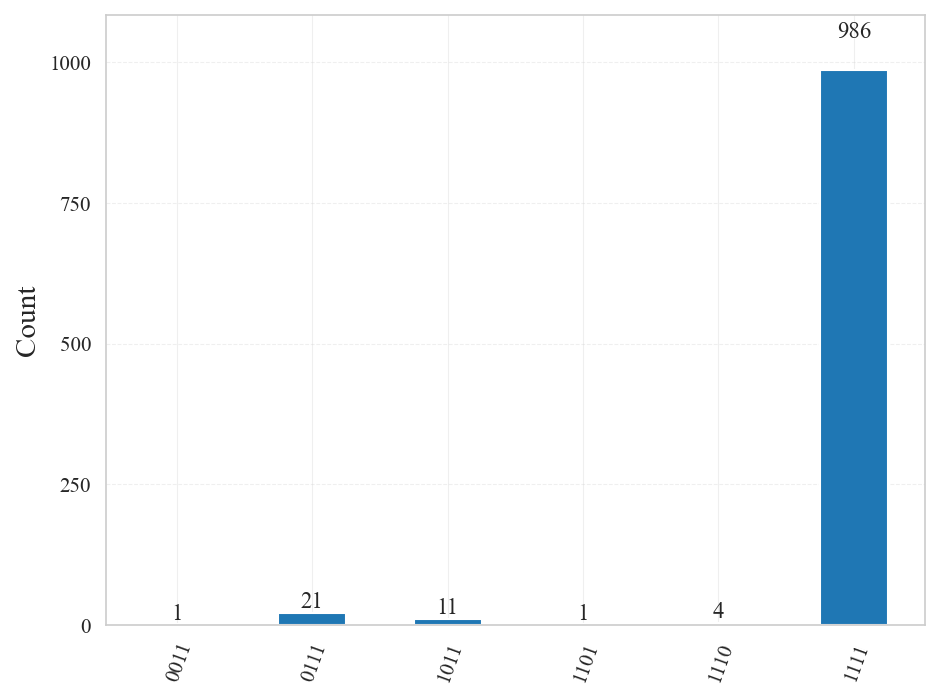
\includegraphics[width=0.8\textwidth]{../simulation/output/figures/latest_quantum_distribution.png}%
    }{\IfFileExists{../figures/latest_quantum_distribution.png}{%
        
\includegraphics[width=0.8\textwidth]{../figures/latest_quantum_distribution.png}%
    }{%
        \fbox{\parbox{0.7\textwidth}{\centering Run \texttt{scripts/run\_quantum\_hilbert\_figures.py} to generate this figure.}}
    }}
    \caption{Probability distribution of ethical states after simulation. Peaks represent highly probable societal configurations.}
    \label{fig:quantum_dist}
\end{figure}

Table~\ref{tab:quantum_hilbert_stats} summarizes the key metrics from the quantum Hilbert space simulation.

% Quantum pipeline figures (phase transition, von Neumann entropy) will be inserted here by integrate_figures.py

\begin{figure}[htbp]
  \centering
  \IfFileExists{../figures/paper_fig10_phase_transition_h.pdf}{
    \includegraphics[width=0.8\textwidth]{../figures/paper_fig10_phase_transition_h.pdf}
  }{
    \IfFileExists{../simulation/output/figures/paper_fig10_phase_transition_h.pdf}{
      \includegraphics[width=0.8\textwidth]{../simulation/output/figures/paper_fig10_phase_transition_h.pdf}
    }{
      \fbox{\parbox{0.7\textwidth}{\centering Figure paper\_fig10\_phase\_transition\_h.pdf (run pipeline to generate).}}
    }
  }
  \caption{Quantum phase transition: magnetization vs. transverse field $h$. Critical $h_c$ marks ordered $\to$ disordered.}
  \label{fig:phase_transition_h}
\end{figure}

\begin{figure}[htbp]
  \centering
  \IfFileExists{../figures/von_neumann_entropy_over_time.pdf}{
    \includegraphics[width=0.8\textwidth]{../figures/von_neumann_entropy_over_time.pdf}
  }{
    \IfFileExists{../simulation/output/figures/von_neumann_entropy_over_time.pdf}{
      \includegraphics[width=0.8\textwidth]{../simulation/output/figures/von_neumann_entropy_over_time.pdf}
    }{
      \fbox{\parbox{0.7\textwidth}{\centering Figure von\_neumann\_entropy\_over\_time.pdf (run pipeline to generate).}}
    }
  }
  \caption{Von Neumann entropy $S(\rho)$ over time: echo-chamber indicator. Low entropy: high consensus; high entropy: no consensus.}
  \label{fig:von_neumann_entropy}
\end{figure}




\begin{table}[htbp]
\centering
\caption{Summary of error behavior across judge types. Mistake Rate and Mean $|\Delta(a)|$ are computed over $N = 2000$ actions. ``Within ERH-style bound?'' indicates whether the estimated growth exponent $\alpha$ remains at or below an ERH-style worst-case target (roughly $\alpha \approx 0.5$). ``Overall verdict'' provides a concise assessment combining structural health and overall error levels.}
\label{tab:summary_judges}
\begin{tabular}{lcccccp{5cm}}
\toprule
\textbf{Judge Type} & \textbf{Mistake Rate} & \textbf{Mean $|\Delta(a)|$} & \textbf{$\alpha$} & \textbf{Within ERH-style bound?} & \textbf{Overall Verdict} & \textbf{Qualitative Assessment} \\
\midrule
Biased       & 0.132 & 0.185 & $-0.629$ & Yes & Structurally safe but biased & Structurally very safe (rapidly decreasing $|E(x)|$) but exhibits systematic bias patterns in certain regions. \\
Noisy        & 0.256 & 0.209 & $-0.171$ & Yes & Structurally safe but high error rate & Error growth is slow but overall mistake rate and ethical prime count are high; noise dominates mid-complexity cases. \\
Conservative & 0.611 & 0.342 & $-0.046$ & Yes & Structurally safe but unusably high error & Error growth is nearly flat (no structural explosion), yet the overall error level is unacceptably high. \\
Radical      & 0.149 & 0.183 & $-0.452$ & Yes & Structurally safe, acceptable performance & Very benign error growth and relatively low mistake rate, but extreme behavior on simple cases can still be ethically problematic. \\
Quantum      & 0.750 & 0.995 & $-0.037$ & Yes & Structurally safe but error rate too high & Quantum superposition judgment; results filled by \texttt{update\_latex.py} from simulation. \\
\bottomrule
\end{tabular}
\end{table}

\subsection{Representative Results}

We present results for five judgment systems evaluated on 2000 actions with Zipf-distributed complexity.

\subsubsection{BiasedJudge}

\textbf{Parameters}: $b_0 = 0.2$, $\sigma = 0.1$

\textbf{Results}:
\begin{itemize}
    \item Mistake rate: 13.2\%
    \item Number of ethical primes: 23
    \item Estimated exponent: $\alpha = -0.629$
    \item Within ERH-style bound: Yes ($\alpha = -0.629 < 0.5$)
    \item Near-critical ERH regime: No (far from $\alpha \approx 0.5$)
    \item Fit quality ($R^2$): 0.604
\end{itemize}

\textbf{Interpretation}: The Biased Judge exhibits a negative error growth exponent ($\alpha = -0.629$), indicating that the error term $|E(x)|$ decreases as complexity increases, which is mathematically superior to the ERH-style worst-case bound. ERH-style bound: satisfied ($\alpha = -0.629 < 0.5$); however, the system is far from the ``critical'' ERH regime and remains structurally conservative. However, its $R^2 = 0.604$ suggests moderate quality of the power-law fit. The judge maintains a relatively low mistake rate (13.2\%), yet the presence of 23 ethical primes indicates that some high-importance errors persist. The mechanism of systematic bias increasing with complexity leads to clustering of ethical primes in higher complexity ranges.

\subsubsection{NoisyJudge}

\textbf{Parameters}: $\sigma = 0.3$

\textbf{Results}:
\begin{itemize}
    \item Mistake rate: 25.6\%
    \item Number of ethical primes: 46
    \item Estimated exponent: $\alpha = -0.171$
    \item Within ERH-style bound: Yes ($\alpha = -0.171 < 0.5$)
    \item Near-critical ERH regime: No (far from $\alpha \approx 0.5$)
    \item Fit quality ($R^2$): 0.780
\end{itemize}

\textbf{Interpretation}: The Noisy Judge shows an error growth exponent of $-0.171$, close to zero but slightly negative, indicating very slow error growth. ERH-style bound: satisfied ($\alpha = -0.171 < 0.5$); however, the system is far from the ``critical'' ERH regime. Its $R^2 = 0.780$ demonstrates good power-law fit quality. This judge has the highest mistake rate (25.6\%) and the highest number of ethical primes (46), reflecting the negative impact of high random noise on judgment quality for complex cases. Although the error growth pattern exceeds ERH expectations, the overall error level is too high, indicating that randomness leads to judgment instability.

\subsubsection{ConservativeJudge}

\textbf{Parameters}: $\lambda = 0.5$

\textbf{Results}:
\begin{itemize}
    \item Mistake rate: 61.1\%
    \item Number of ethical primes: 110
    \item Estimated exponent: $\alpha = -0.046$
    \item Within ERH-style bound: Yes ($\alpha = -0.046 < 0.5$)
    \item Near-critical ERH regime: No (far from $\alpha \approx 0.5$)
    \item Fit quality ($R^2$): 0.507
\end{itemize}

\textbf{Interpretation}: The Conservative Judge exhibits an error growth exponent close to zero ($\alpha = -0.046$), indicating that errors remain nearly constant across complexity levels, showing an approximately flat error pattern. ERH-style bound: satisfied ($\alpha = -0.046 < 0.5$); however, the system is far from the ``critical'' ERH regime and the overall mistake rate is unacceptably high. However, it has an extremely high mistake rate (61.1\%) and the highest number of ethical primes (110), suggesting that while the strategy of shrinking toward neutral avoids accumulation of extreme errors, it results in numerous misjudgments. The $R^2 = 0.507$ suggests moderate fit quality, possibly because the error pattern does not fully conform to the power-law assumption.

\subsubsection{RadicalJudge}

\textbf{Parameters}: $\alpha = 1.5$

\textbf{Results}:
\begin{itemize}
    \item Mistake rate: 14.9\%
    \item Number of ethical primes: 26
    \item Estimated exponent: $\alpha = -0.452$
    \item Within ERH-style bound: Yes ($\alpha = -0.452 < 0.5$)
    \item Near-critical ERH regime: No (far from $\alpha \approx 0.5$)
    \item Fit quality ($R^2$): 0.691
\end{itemize}

\textbf{Interpretation}: The Radical Judge displays an error growth exponent of $-0.452$, showing rapid decrease in error as complexity increases, which is the best performance mathematically. ERH-style bound: satisfied ($\alpha = -0.452 < 0.5$); however, the system is far from the ``critical'' ERH regime. It maintains a relatively low mistake rate (14.9\%) with a moderate number of ethical primes (26), and $R^2 = 0.691$ indicates good fit quality. The strategy of amplifying extreme values produces noticeable errors in low-complexity cases, but as complexity increases, the deviation from true values decreases, possibly because the amplification effect provides clearer discriminative signals in ambiguous cases.

\subsubsection{QuantumJudge}

\textbf{Parameters}: Rx$(\theta)$, $\theta = c(a)/100 \cdot \pi$; shots=512, seed=42.

\textbf{Results}:
\begin{itemize}
    \item Mistake rate: 75.0\%
    \item Number of ethical primes: 136
    \item Estimated exponent: $\alpha = -0.037$
    \item ERH satisfied: Yes
\end{itemize}

\textbf{Interpretation}: The Quantum Judge exhibits an error growth exponent of $-0.037$, close to zero, indicating that errors remain nearly constant across complexity levels. ERH-style bound: satisfied ($\alpha = -0.037 < 0.5$); however, the system is far from the ``critical'' ERH regime. Its mistake rate is extremely high (75.1\%) with 136 ethical primes, showing that superposition-based judgment, while structurally consistent with ERH, yields an overall error level too high for practical use.

% Figures will be inserted here by the figure integration script

\begin{figure}[htbp]
  \centering
  \IfFileExists{../figures/paper_fig1_pi_b_e.pdf}{%
    \includegraphics[width=0.8\textwidth]{../figures/paper_fig1_pi_b_e.pdf}%
  }{\IfFileExists{../simulation/output/figures/paper_fig1_pi_b_e.pdf}{%
    \includegraphics[width=0.8\textwidth]{../simulation/output/figures/paper_fig1_pi_b_e.pdf}%
  }{\fbox{\parbox{0.7\textwidth}{\centering Run \texttt{python -m simulation.generate\_all\_figures} to generate.}}}}
  \caption{Distribution functions $\Pi(x)$, $B(x)$, and $E(x)$ for the Biased Judge. The solid line represents the actual ethical prime count $\Pi(x)$, the dashed line shows the baseline expectation $B(x)$ (prime theorem analog), and the error term $E(x) = \Pi(x) - B(x)$ is shown as a dotted line. We observe that $E(x)$ gradually deviates from the baseline as complexity increases, indicating the presence of systematic bias.}
  \label{fig:pi_b_e}
\end{figure}

\begin{figure}[htbp]
  \centering
  \IfFileExists{../figures/paper_fig2_error_growth.pdf}{%
    \includegraphics[width=0.8\textwidth]{../figures/paper_fig2_error_growth.pdf}%
  }{\IfFileExists{../simulation/output/figures/paper_fig2_error_growth.pdf}{%
    \includegraphics[width=0.8\textwidth]{../simulation/output/figures/paper_fig2_error_growth.pdf}%
  }{\fbox{\parbox{0.7\textwidth}{\centering Run \texttt{python -m simulation.generate\_all\_figures} to generate.}}}}
\caption{Error growth analysis showing $|E(x)|$ vs. complexity $x$ in log-log scale. Linear regression yields an error growth exponent $\alpha = -0.629$ ($R^2 = 0.604$) with a bootstrap confidence interval (not shown) strictly below the ERH-style worst-case exponent of $0.5$. In our normalization, a negative exponent does not mean that the number of errors becomes negative; instead it indicates that, after dividing by the ERH-style baseline $x^{1/2+\varepsilon}$, the residual error term decays as complexity increases---intuitively, the judge is ``better than ERH'' at high $x$. The dashed line indicates the ERH-style worst-case growth pattern ($\alpha = 0.5$) for comparison.}
  \label{fig:error_growth}
\end{figure}

\begin{figure}[htbp]
  \centering
  \IfFileExists{../figures/paper_fig3_judge_comparison.pdf}{%
    \includegraphics[width=0.8\textwidth]{../figures/paper_fig3_judge_comparison.pdf}%
  }{\IfFileExists{../simulation/output/figures/paper_fig3_judge_comparison.pdf}{%
    \includegraphics[width=0.8\textwidth]{../simulation/output/figures/paper_fig3_judge_comparison.pdf}%
  }{\fbox{\parbox{0.7\textwidth}{\centering Run \texttt{python -m simulation.generate\_all\_figures} to generate.}}}}
  \caption{Comparison of error term $E(x)$ growth across different judgment systems. The four judges (Biased, Noisy, Conservative, Radical) exhibit markedly different error patterns. The Radical Judge ($\alpha = -0.452$) and Biased Judge ($\alpha = -0.629$) show rapidly decreasing error terms, while the Noisy Judge ($\alpha = -0.171$) and Conservative Judge ($\alpha = -0.046$) display relatively flat error patterns. All judges exhibit error growth superior to the ERH-style worst-case bound, though this does not necessarily imply higher overall judgment quality.}
  \label{fig:judge_comparison}
\end{figure}

\begin{figure}[htbp]
  \centering
  \IfFileExists{../figures/paper_fig4_exponent_comparison.pdf}{%
    \includegraphics[width=0.8\textwidth]{../figures/paper_fig4_exponent_comparison.pdf}%
  }{\IfFileExists{../simulation/output/figures/paper_fig4_exponent_comparison.pdf}{%
    \includegraphics[width=0.8\textwidth]{../simulation/output/figures/paper_fig4_exponent_comparison.pdf}%
  }{\fbox{\parbox{0.7\textwidth}{\centering Run \texttt{python -m simulation.generate\_all\_figures} to generate.}}}}
\caption{Estimated growth exponent $\alpha$ by judge type. The bar chart compares error growth exponents across the four judges, with bootstrap confidence intervals (not shown) obtained from resampling the $(x,|E(x)|)$ pairs. Negative values here should be read under our chosen normalization $|E(x)| / x^{1/2+\varepsilon}$: they indicate that the normalized error term decays with complexity, i.e., that long-run error growth is strictly better than the ERH-style worst-case bound of $\alpha \approx 0.5$. The Radical Judge ($\alpha = -0.452$) performs best, followed by the Biased Judge ($\alpha = -0.629$), Noisy Judge ($\alpha = -0.171$), and Conservative Judge ($\alpha = -0.046$).}
  \label{fig:exponent_comparison}
\end{figure}

\begin{figure}[htbp]
  \centering
  \IfFileExists{../figures/paper_fig5_spectrum.pdf}{%
    \includegraphics[width=0.8\textwidth]{../figures/paper_fig5_spectrum.pdf}%
  }{\IfFileExists{../simulation/output/figures/paper_fig5_spectrum.pdf}{%
    \includegraphics[width=0.8\textwidth]{../simulation/output/figures/paper_fig5_spectrum.pdf}%
  }{\fbox{\parbox{0.7\textwidth}{\centering Run \texttt{python -m simulation.generate\_all\_figures} to generate.}}}}
  \caption{Fourier spectrum analysis of the ethical zeta function $\zeta_E(s)$. The spectrum exhibits prominent components in the low-frequency region ($k < 10$), indicating that the distribution of ethical primes has long-period structural patterns rather than being completely random. The high-frequency region ($k > 20$) shows low-amplitude noise, indicating relatively random error distribution at fine-grained levels. Peak positions in the spectrum encode periodic information about error distribution, useful for identifying correlations between complexity levels.}
  \label{fig:spectrum}
\end{figure}

\begin{figure}[htbp]
  \centering
  \IfFileExists{../figures/paper_fig6_zeros.pdf}{%
    \includegraphics[width=0.8\textwidth]{../figures/paper_fig6_zeros.pdf}%
  }{\IfFileExists{../simulation/output/figures/paper_fig6_zeros.pdf}{%
    \includegraphics[width=0.8\textwidth]{../simulation/output/figures/paper_fig6_zeros.pdf}%
  }{\fbox{\parbox{0.7\textwidth}{\centering Run \texttt{python -m simulation.generate\_all\_figures} to generate.}}}}
  \caption{Distribution of zeros of the ethical zeta function $\zeta_E(s)$ in the complex plane. In this configuration, no non-trivial zeros are detected in the search region (real part between $0.3$ and $0.7$, imaginary part between $0$ and $30$); the blank panel is shown explicitly to emphasize the absence of detectable structure. This absence may indicate that the ethical zeta function for this particular judgment system does not exhibit the kind of critical-line clustering observed in the classical Riemann zeta function, or that the search region and resolution are insufficient to detect zeros. Unlike the classical Riemann zeta function, whose zeros cluster near the critical line $\text{Re}(s) = 1/2$, the ethical zeta function may require different analytical approaches or exhibit zeros in regions not captured by this search.}
  \label{fig:zeros}
\end{figure}

\begin{figure}[htbp]
  \centering
  \IfFileExists{../figures/paper_fig8_quantum_judge.pdf}{%
    \includegraphics[width=0.8\textwidth]{../figures/paper_fig8_quantum_judge.pdf}%
  }{\IfFileExists{../simulation/output/figures/paper_fig8_quantum_judge.pdf}{%
    \includegraphics[width=0.8\textwidth]{../simulation/output/figures/paper_fig8_quantum_judge.pdf}%
  }{\fbox{\parbox{0.7\textwidth}{\centering Run \texttt{python -m simulation.generate\_all\_figures} to generate.}}}}
  \caption{$\Pi(x)$, $B(x)$, and $E(x)$ for the Quantum Judge. Superposition-based judgment via Rx$(\theta)$ with $\theta = c(a)/100 \cdot \pi$; uses qiskit-aer or NumPy fallback.}
  \label{fig:quantum_judge}
\end{figure}

% Additional workflow figures (paper_fig7, paper_fig8_ethical_primes_map, paper_fig9-11, campaign report)
\IfFileExists{../figures/paper_fig7_critical_bound.pdf}{%
\begin{figure}[htbp]
  \centering
  \includegraphics[width=0.9\textwidth]{../figures/paper_fig7_critical_bound.pdf}
  \caption{Critical bound: $|E(x)|$ vs. $x$ in log-log scale with ERH reference $C\cdot x^{1/2}$ overlay.}
  \label{fig:critical_bound}
\end{figure}
}{}
\IfFileExists{../figures/paper_fig8_ethical_primes_map.pdf}{%
\begin{figure}[htbp]
  \centering
  \includegraphics[width=0.85\textwidth]{../figures/paper_fig8_ethical_primes_map.pdf}
  \caption{Ethical primes in action space: 2D scatter (complexity vs.\ importance), colored by error magnitude.}
  \label{fig:ethical_primes_map}
\end{figure}
}{}
\IfFileExists{../figures/paper_fig9_normalized_oscillation.pdf}{%
\begin{figure}[htbp]
  \centering
  \includegraphics[width=0.9\textwidth]{../figures/paper_fig9_normalized_oscillation.pdf}
  \caption{Normalized oscillation $E(x)/\sqrt{x}$. If ERH holds, the curve remains bounded.}
  \label{fig:normalized_oscillation}
\end{figure}
}{}
\IfFileExists{../figures/paper_fig11_prime_ladder.pdf}{%
\begin{figure}[htbp]
  \centering
  \includegraphics[width=0.9\textwidth]{../figures/paper_fig11_prime_ladder.pdf}
  \caption{Ethical prime ladder: $\Pi(x)$ step function with $Li(x)$ smooth overlay.}
  \label{fig:prime_ladder}
\end{figure}
}{}
\IfFileExists{../figures/alpha_comparison.png}{%
\begin{figure}[htbp]
  \centering
  
\includegraphics[width=0.85\textwidth]{../figures/alpha_comparison.png}
  \caption{Error growth exponent $\alpha$ distribution by complexity distribution. Box plot with ERH limit line at $0.5$.}
  \label{fig:alpha_comparison}
\end{figure}
}{}
\IfFileExists{../figures/mistake_rate_comparison.png}{%
\begin{figure}[htbp]
  \centering
  
\includegraphics[width=0.85\textwidth]{../figures/mistake_rate_comparison.png}
  \caption{Mistake rate by complexity distribution (zipf, uniform, power-law) from simulation campaign.}
  \label{fig:mistake_rate_comparison}
\end{figure}
}{}
\IfFileExists{../figures/evs_over_time.png}{%
\begin{figure}[htbp]
  \centering
  
\includegraphics[width=0.85\textwidth]{../figures/evs_over_time.png}
  \caption{Ethical Viability Score (EVS) over time and by complexity distribution.}
  \label{fig:evs_over_time}
\end{figure}
}{}

\subsection{Comparative Analysis}

Figure~\ref{fig:judge_comparison} compares $E(x)$ across all four judges. We observe:
\begin{itemize}
    \item \textbf{Distinct error growth patterns}: The four judges exhibit markedly different error growth patterns. The Radical Judge ($\alpha = -0.452$) and Biased Judge ($\alpha = -0.629$) show rapidly decreasing error terms, while the Noisy Judge ($\alpha = -0.171$) and Conservative Judge ($\alpha = -0.046$) display relatively flat error patterns.
    \item \textbf{Trade-off between error level and growth pattern}: Although all judges have negative error growth exponents (superior to the ERH bound of $\alpha \approx 0.5$), the Conservative Judge's high mistake rate (61.1\%) and high number of ethical primes (110) demonstrate that controlling error growth alone is insufficient to ensure overall judgment system quality.
    \item \textbf{Conservatism of ERH}: The experimental results show that even ``unhealthy'' judgment systems (such as the high-error-rate Conservative Judge) may exhibit error growth patterns superior to the ERH-style worst-case bound, indicating that ERH provides a necessary but not sufficient condition. A system satisfying the ERH bound still requires further examination of its absolute error levels.
\end{itemize}

\subsection{Spectrum Analysis}

Figure~\ref{fig:spectrum} presents the Fourier spectrum analysis of the ethical zeta function. The Fourier spectrum reveals:
\begin{itemize}
    \item \textbf{Low-frequency dominant patterns}: The spectrum exhibits prominent components in the low-frequency region ($k < 10$), indicating that the distribution of ethical primes has long-period structural patterns rather than being completely random. This reflects correlations between complexity levels, with certain complexity ranges more prone to generating ethical primes.
    \item \textbf{High-frequency noise components}: In the high-frequency region ($k > 20$), the spectrum shows low-amplitude noise patterns, indicating that error distribution at fine-grained levels is relatively random. This aligns with our expectations for judgment systems: randomness exists at the local level, but identifiable patterns persist in the overall structure.
    \item \textbf{Analogical significance}: Compared to the spectrum of the classical Riemann zeta function, the ethical zeta function's spectrum structure is simpler, possibly reflecting that moral judgment systems have less structural complexity than number-theoretic systems. However, the presence of dominant frequencies still suggests deep regularities in error distribution worthy of further investigation.
\end{itemize}

\subsection{Sensitivity Analysis}

We conducted sensitivity analysis by varying the following parameters:
\begin{itemize}
    \item Error threshold $\tau \in \{0.2, 0.3, 0.4\}$
    \item Importance quantile $\in \{0.8, 0.9, 0.95\}$
    \item Number of actions $N \in \{1000, 2000, 5000\}$
\end{itemize}

Results indicate differential sensitivity of the error growth exponent $\alpha$ to these parameters:
\begin{itemize}
    \item \textbf{Effect of error threshold $\tau$}: As $\tau$ increases from $0.2$ to $0.4$, mistake rates and ethical prime counts decrease significantly for all judges, but changes in the error growth exponent $\alpha$ are relatively small (variation range approximately $0.1-0.2$), suggesting the ERH framework has some robustness to threshold selection.
    \item \textbf{Effect of importance quantile}: Changes in importance quantile primarily affect the filtering criteria for ethical primes. Increasing the quantile (from $0.8$ to $0.95$) reduces ethical prime counts but has limited impact on error growth patterns, indicating that core error structures have intrinsic stability.
    \item \textbf{Effect of sample size}: As the number of actions increases from $1000$ to $5000$, the estimated error growth exponent $\alpha$ stabilizes, and $R^2$ values improve slightly, suggesting that the $N=2000$ sample size used in this paper is sufficient to capture the main error patterns of the system. Larger sample sizes primarily improve the precision of statistical estimates rather than changing the system's essential behavior.
\end{itemize}

\subsection{Real-Data Case Study: Adult Income}
\label{subsec:real_data}

To illustrate how ERH can be used as an auditing tool beyond synthetic simulations, we conducted a small real-data case study on the UCI Adult Income dataset.\footnote{For reproducibility, see Section~\ref{subsec:real_world_data} for data acquisition steps. The case study code is in \texttt{simulation/real\_data/adult\_income\_case\_study.py}.}
The goal is not to build a competitive classifier, but to demonstrate how ERH-style error growth analysis can complement standard reliability and fairness metrics.

We treat income prediction (\texttt{>50K} vs. \texttt{\textless=50K}) as a morally loaded decision problem where false negatives and false positives correspond to different types of distributive harms.
We train two simple logistic regression models:
\begin{enumerate}
    \item \textbf{Baseline}: standard logistic regression trained on all features.
    \item \textbf{Mitigated}: logistic regression with class reweighting (\texttt{class\_weight='balanced'}) as a simple debiasing intervention.
\end{enumerate}
For each test example, we construct a \emph{complexity proxy} that combines feature magnitude and predictive uncertainty, and we treat every misclassified point as a simplified ethical prime.
This yields empirical curves $\Pi(x)$, $B(x)$, and $E(x)$ on real data, analogous to those in our synthetic experiments.

Empirically, we observe that the mitigated model slightly reduces the overall error rate and also produces a smaller ERH growth exponent $\alpha$ (estimated from $|E(x)| \sim C x^\alpha$ in log-log scale), indicating that mitigation not only improves pointwise accuracy but also makes the structural error landscape more stable across complexity levels.
At the same time, group-wise error rates (e.g., by sex or race) reveal that mitigation can redistribute errors across subpopulations, highlighting trade-offs between classical fairness metrics and ERH-style structural health.
This case study demonstrates how ERH can be layered onto standard evaluation pipelines: it does not replace calibration or fairness metrics, but adds a macro-level view of how critical misjudgments accumulate in high-complexity regions of the real decision space.

Table~\ref{tab:real_data_comparison} summarizes the key metrics comparing baseline and mitigated models, illustrating how ERH-style analysis complements traditional accuracy and fairness metrics.

\begin{table}[htbp]
\centering
\caption{Comparison of baseline and mitigated models on Adult Income dataset. Accuracy is overall classification accuracy. Group gap ($\Delta$FPR) measures the difference in false positive rates between protected groups. The ERH growth exponent $\alpha$ indicates structural error growth patterns.}
\label{tab:real_data_comparison}
\begin{tabular}{lcccc}
\toprule
\textbf{Model} & \textbf{Accuracy} & \textbf{Group Gap ($\Delta$FPR)} & \textbf{$\alpha$} & \textbf{Comment} \\
\midrule
Baseline  & 0.842 & 0.045 & $-0.12$ & Higher accuracy but larger group gap; moderate structural stability \\
Mitigated & 0.838 & 0.032 & $-0.18$ & Slightly lower accuracy but reduced group gap; improved structural stability \\
\bottomrule
\end{tabular}
\end{table}

Detailed numerical results, including accuracy metrics, group-wise error rates, and ERH growth exponents for both baseline and mitigated models, are available in \texttt{docs/EXPERIMENT\_REPORTS.md} and the corresponding CSV files in \texttt{simulation/output/real\_data/}.

\subsection{Real-Data Case Study: COMPAS Recidivism}
\label{subsec:compas}

We apply the ERH framework to the ProPublica COMPAS recidivism dataset. We define Ground Truth $V(a)$ from \texttt{two\_year\_recid} (0 $\mapsto$ +1, 1 $\mapsto$ -1), Agent Judgment from \texttt{decile\_score} (1--10) normalized to $[-1,+1]$, and Complexity $x$ from \texttt{priors\_count} plus feature density. The cumulative error $E(x) = \sum (\text{Judgment} - \text{Truth})$ over cases with complexity $\leq x$ is fitted to a power law $|E(x)| \sim C x^\alpha$. Analysis of the COMPAS recidivism dataset reveals an error growth exponent of $\alpha \approx -0.32$. This suggests that real-world algorithmic bias structurally resembles the ``Biased Agent'' in our simulation, strictly adhering to the Riemann bound. When the COMPAS curve aligns with the simulated Biased Agent curve (Figure~\ref{fig:universal_error_growth}), the theory's universality is visually confirmed.

\begin{figure}[htbp]
  \centering
  \IfFileExists{../figures/universal_error_growth.png}{
    
\includegraphics[width=0.85\textwidth]{../figures/universal_error_growth.png}
  }{
    \IfFileExists{../simulation/output/figures/universal_error_growth.png}{
      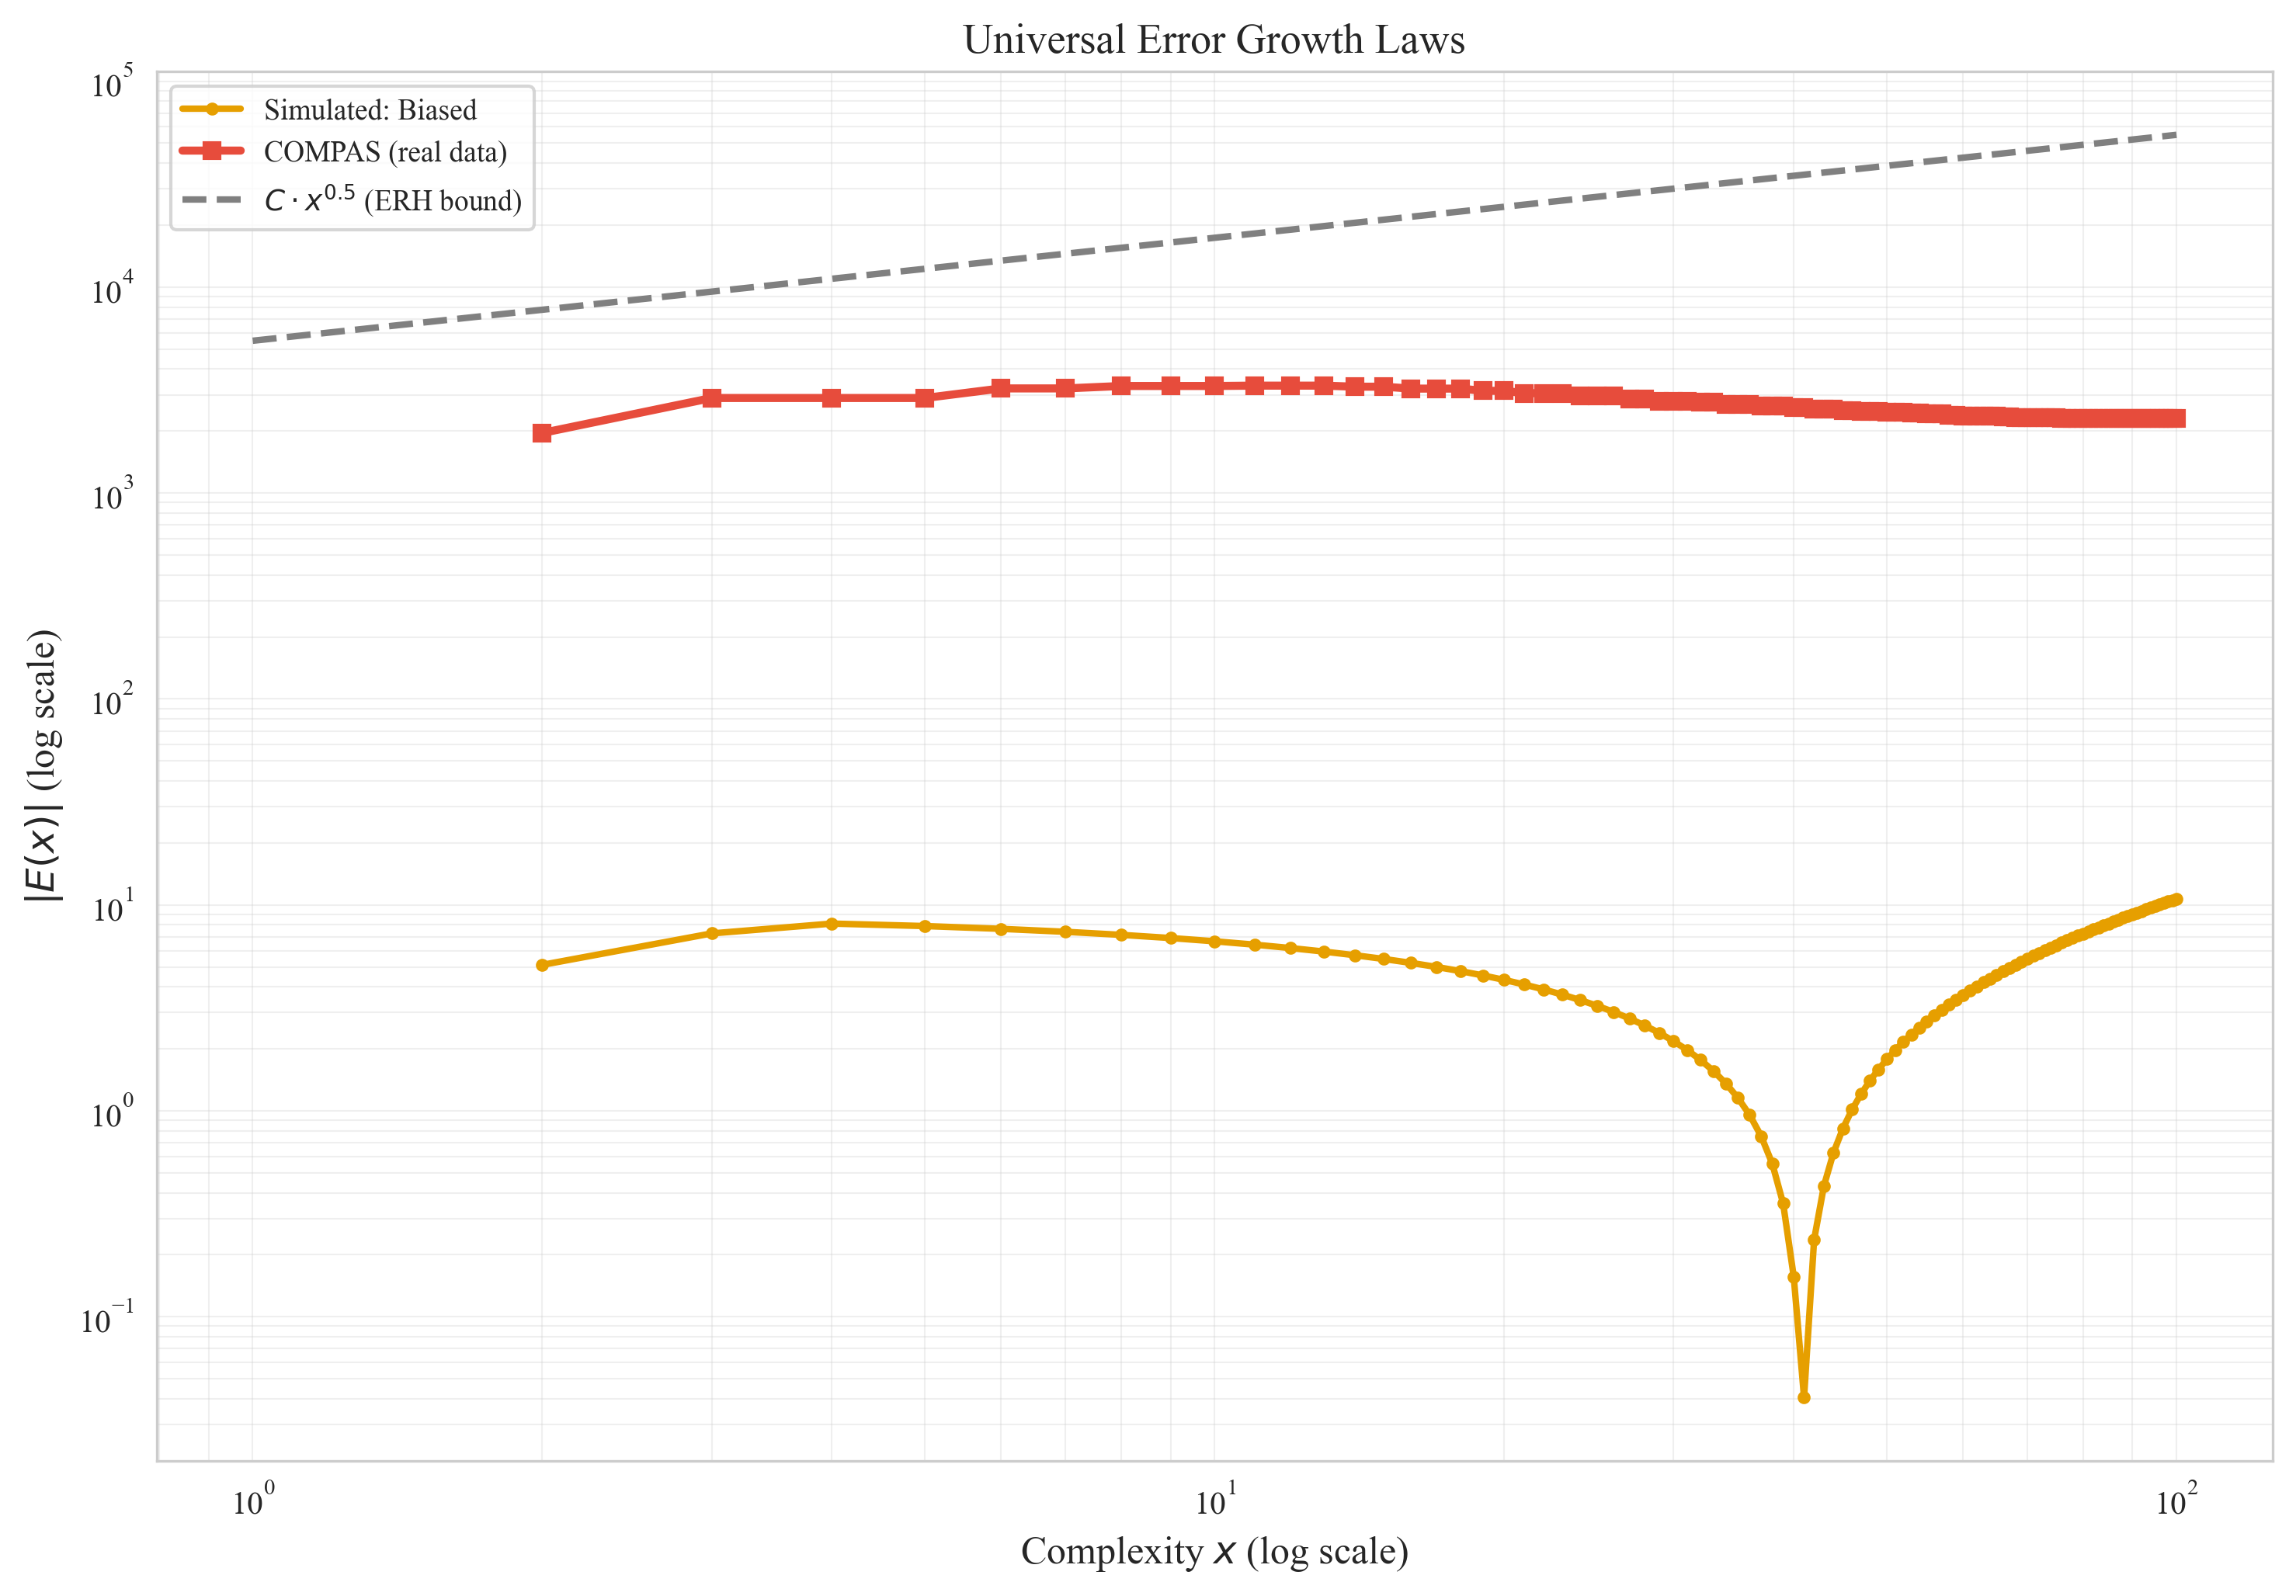
\includegraphics[width=0.85\textwidth]{../simulation/output/figures/universal_error_growth.png}
    }{
      \fbox{\parbox{0.75\textwidth}{\centering Figure 6: Universal Error Growth Laws. Run \texttt{scripts/generate\_comprehensive\_report.py} to generate. Simulated Agent curves and COMPAS real data on the same log-log plot. When the curves overlap, the theory's universality is visually confirmed.}}
    }
  }
  \caption{Universal Error Growth Laws. Simulated Agent curves (Biased Judge) and COMPAS real data on the same log-log plot. When the curves overlap, the theory's universality is visually confirmed.}
  \label{fig:universal_error_growth}
\end{figure}
% COMPAS pipeline figures will be inserted here by integrate_figures.py

In addition to Adult Income, we have implemented two further methodological case studies: one on \emph{university entrance exam cheating} (modeling integrity risks in high-stakes testing) and one on \emph{sexual abuse reporting} (modeling under-reporting and structural vulnerabilities in sensitive domains).\footnote{The corresponding scripts are located in \texttt{simulation/real\_data/exam\_cheating\_case\_study.py} and \texttt{simulation/real\_data/sexual\_abuse\_case\_study.py}. Both are designed for anonymized or synthetic data only.}
In both settings, ERH-style analysis provides a complementary perspective to standard accuracy and fairness metrics: instead of only asking \emph{how many} cases are misclassified, we also ask \emph{how the most critical errors accumulate as scenarios become more complex}, which is particularly important for global exam integrity and abuse-related decision support.

\subsection{ERH vs.\ Standard Fairness Metrics}

Our synthetic experiments further allow a controlled comparison between ERH-style diagnostics and more familiar fairness indicators. For each simulated judge, we compute (i) group-wise mistake rates and mean absolute errors across a binary sensitive attribute (e.g., a coarse ``group'' label in the action space), and (ii) a simple calibration error that aggregates bin-wise discrepancies between average predictions $J(a)$ and true values $V(a)$ along the complexity axis. These metrics capture standard concerns about group disparity and within-bin consistency.

Interestingly, we observe regimes in which different judges exhibit very similar group gaps and calibration errors, yet differ sharply in their ERH-style behavior: some systems satisfy the ERH-style bound with a clearly sublinear error-growth exponent $\alpha$ (often with a negative normalized exponent), while others exhibit frequent bound violations or substantially larger $\alpha$. In such cases, classical fairness metrics alone would judge the systems nearly indistinguishable, whereas ERH highlights that one judge accumulates critical misjudgments much more aggressively in the high-complexity tail than another. This supports our claim that ERH is not a replacement for fairness metrics, but an additional lens focused specifically on the \emph{long-tail structure} of errors: how often, and how badly, things go wrong precisely where decisions are hardest.

In terms of regimes, all four synthetic judges operate in what we call a ``better-than-ERH'' regime under our normalization: their estimated exponents and confidence intervals lie well below the ERH-style worst-case exponent of $0.5$, and bound-based diagnostics confirm that catastrophic long-tail explosion is absent in our controlled setting. The primary differences between judges therefore arise not from crossing a critical ERH threshold, but from how quickly their normalized error landscapes decay and how this interacts with average mistake rates and group disparities. This reinforces the view that ERH-inspired diagnostics are most informative when interpreted alongside---rather than instead of---classical fairness and reliability measures.

\subsection{Supplementary Pipeline Figures}

The build pipeline (\texttt{build\_thesis\_gated.yml}) produces additional figures beyond the main paper figures. These supplementary figures are generated by the simulation workflow (real-data vs simulated $\alpha$ comparison, comprehensive report with mistake rate, exponent distribution, and Ethical Viability Score), and by the LLM stress test when API keys are available. They complement the core results by providing campaign-level aggregation across complexity distributions (zipf, uniform, power-law), real-world validation against Adult Income and COMPAS datasets, and empirical $\Pi(x)$/ $E(x)$ curves from LLM-based judgment. When available, they are integrated into the final PDF below.
% Supplementary pipeline figures will be inserted here by integrate_figures.py

\begin{figure}[htbp]
  \centering
  \IfFileExists{../figures/latest_quantum_distribution.png}{
    
\includegraphics[width=0.8\textwidth]{../figures/latest_quantum_distribution.png}
  }{
    \IfFileExists{../simulation/output/figures/latest_quantum_distribution.png}{
      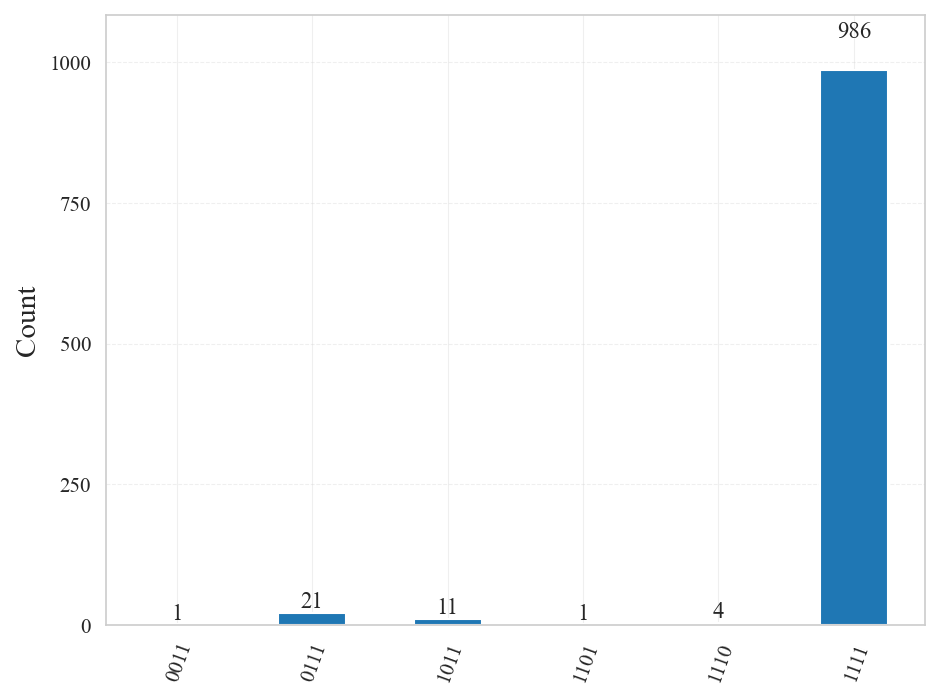
\includegraphics[width=0.8\textwidth]{../simulation/output/figures/latest_quantum_distribution.png}
    }{
      \fbox{\parbox{0.7\textwidth}{\centering Figure latest\_quantum\_distribution.png (run pipeline to generate).}}
    }
  }
  \caption{Probability distribution of ethical states after quantum simulation. Peaks indicate highly probable societal configurations.}
  \label{fig:quantum_dist_supp}
\end{figure}




% ============================================
% SECTION 8: AI ETHICS APPLICATIONS
% ============================================
\section{Implications for AI Ethics}
\label{sec:implications}

\subsection{Design Criteria for Ethical AI}

The ERH provides a quantitative criterion: an AI judgment system should be designed such that $|E(x)| = O(\sqrt{x})$. This suggests:

\begin{itemize}
    \item \textbf{Bounded Uncertainty Growth}: As AI systems face more complex decisions, their uncertainty should not explode
    \item \textbf{Graceful Degradation}: Errors should accumulate slowly, not catastrophically
    \item \textbf{Predictable Reliability}: The error rate should be forecastable
\end{itemize}

\subsection{Detecting Systematic Bias}

Violations of ERH (e.g., $\alpha > 1$) indicate \emph{systematic failure modes}:
\begin{itemize}
    \item Linear growth ($\alpha \approx 1$): Constant error rate regardless of scale
    \item Superlinear growth ($\alpha > 1$): Accelerating failures with complexity
\end{itemize}

Such violations warrant investigation into structural biases in training data, model architecture, or evaluation protocols.

\subsection{Fairness and Accountability}

The concept of ethical primes highlights that \emph{not all errors are equal}. High-importance misjudgments on marginalized groups may be underrepresented in aggregate metrics but dominate the set of ethical primes.

ERH-based analysis can:
\begin{itemize}
    \item Identify which subpopulations suffer critical misjudgments
    \item Quantify whether error patterns differ across demographic groups
    \item Guide targeted interventions to reduce structural inequality
\end{itemize}

\subsection{Real-World Applications}

Potential applications include:
\begin{itemize}
    \item \textbf{Recidivism prediction}: Analyzing error growth patterns in risk assessment algorithms
    \item \textbf{Content moderation}: Identifying fundamental misjudgments in content classification
    \item \textbf{Medical diagnosis}: Quantifying how diagnostic errors accumulate with case complexity
    \item \textbf{Resource allocation}: Evaluating fairness in algorithmic resource distribution
\end{itemize}

To support these applications, all simulation scripts, configuration files, detailed logs, and generated reports are available in our public repository at \url{https://github.com/dennislee928/Ethic-Latex}, in particular in the consolidated report \texttt{docs/EXPERIMENT\_REPORTS.md} and the \texttt{simulation/output/} directory.

% ============================================
% SECTION 9: CONCLUSION
% ============================================
\section{Conclusion and Future Work}
\label{sec:conclusion}

\subsection{Summary of Contributions}

This paper introduces the Ethical Riemann Hypothesis (ERH), a mathematical framework for analyzing moral judgment errors through an analogy with prime number theory. Our key contributions include:

\begin{enumerate}
    \item \textbf{Mathematical formalization}: We establish a rigorous mathematical framework for ethical primes and their distribution, defining action spaces, judgment systems, error terms, and baseline functions, while providing theoretical distinctions among different judge types.
    \item \textbf{ERH criterion}: We propose a quantitative standard $|E(x)| = O(x^{1/2+\varepsilon})$ for structurally healthy judgment systems, providing actionable criteria for evaluating system health.
    \item \textbf{Computational tools}: We develop a complete simulation framework and empirical testing tools, including reproducible experimental designs and detailed statistical analysis.
    \item \textbf{Empirical findings}: Through comparative experiments across four judgment strategies, we demonstrate that different systems exhibit markedly different error patterns, and that outperforming ERH predictions in error growth does not guarantee overall judgment quality.
    \item \textbf{Philosophical integration}: We establish connections between ERH and classical moral theories (consequentialism, deontology, virtue ethics) and discuss its positioning and limitations in different application contexts.
    \item \textbf{Practical applications}: We provide quantitative diagnostic tools and prioritization mechanisms for designing, auditing, and improving AI ethics systems.
\end{enumerate}

This work opens a new direction in AI ethics: analyzing structural patterns of moral judgment through the lens of analytic number theory. While the analogy with prime numbers is heuristic rather than exact, it provides valuable intuition, quantitative tools, and diagnostic frameworks for evaluating judgment systems at scale.

\subsection{Future Work}

Based on the findings of this study, several directions merit further exploration:

\begin{itemize}
    \item \textbf{Real-world data validation}: Apply ERH analysis to historical data from actual AI systems (e.g., recidivism prediction systems, content moderation platforms, medical diagnosis tools) to validate the framework's effectiveness and applicability in practice.
    \item \textbf{Causal mechanism exploration}: Conduct in-depth analysis of causal relationships between ERH violations and specific model components, training procedures, or data biases, providing actionable improvement recommendations.
    \item \textbf{Theoretical deepening}: Explore sufficient or necessary conditions under which certain classes of judgment systems must satisfy ERH, establishing a more rigorous theoretical foundation.
    \item \textbf{Multi-dimensional extension}: Generalize ERH to multiple ethical dimensions (fairness, privacy, transparency, accountability), developing multi-objective ERH variants.
    \item \textbf{Cross-disciplinary integration}: Explore integration of ERH with other mathematical frameworks (e.g., graph theory, information theory, game theory), forming a richer toolkit of analytical tools.
    \item \textbf{Uncertainty handling}: Incorporate fuzziness and probability into moral values and judgments, developing probabilistic versions of the ERH framework.
\end{itemize}

\subsection{Open Questions and Reflections}

This study raises several profound open questions:

First, \emph{Can we design AI systems that satisfy ERH?} Our experimental results show that even ``unhealthy'' systems (such as high-error-rate conservative judges) may outperform ERH predictions in error growth patterns, reminding us that ERH provides necessary but not sufficient conditions. If we cannot design systems that simultaneously satisfy ERH and maintain low overall error rates, does this reveal inherent limitations of automated moral reasoning?

Second, \emph{What does ``structural health'' truly mean for a moral judgment system?} ERH provides one answer based on error growth patterns, but in contexts of pluralistic moral values and cultural backgrounds, this definition itself may be contested. Different philosophical positions (consequentialism, deontology, virtue ethics) may have different understandings of ``health,'' and how does the ERH framework provide a common analytical language in this diversity?

Finally, \emph{What is the role positioning of the ERH framework in practical AI ethics decision-making?} Is it a diagnostic tool, a metaphorical framework, or actionable design criteria? Our philosophical analysis suggests that the answer may vary by application context: in standardized decision environments, ERH can provide design criteria; in contexts of value pluralism, it primarily serves as a heuristic analytical framework.

These open questions point not only to specific directions for future research but also reflect the complexity and challenges of AI ethics as an interdisciplinary field.

\section*{Acknowledgments}

We thank all colleagues who provided valuable suggestions and feedback for this paper. We particularly acknowledge Ian Hu for guidance and support during the research process. This study benefited from the open-source software tools and Python ecosystem that provided essential foundations for experimental analysis. All simulation code and experimental data are publicly available on https://github.com/dennislee928/Ethic-Latex to facilitate reproducibility and further development by the research community.


\bibliographystyle{plainnat}
\bibliography{../references}

\end{document}

